\documentclass[aspectratio=169]{beamer}

% ============================================
% PACOTES ADICIONAIS
% ============================================
\usepackage[utf8]{inputenc}
\usepackage[T1]{fontenc}
\usepackage{amsmath}
\usepackage{amsfonts}
\usepackage{amssymb}
\usepackage{graphicx}
\usepackage{cite}
\usepackage{url}
\usepackage{hyperref}
\usepackage{ifthen}
\usepackage{bm}
\usepackage{array}
\usepackage{cancel}
\usepackage{tikz}
\usepackage{circuitikz}

% ============================================
% VARIÁVEIS DE CONFIGURAÇÃO
% ============================================

% --- Informações do Autor ---
\newcommand{\autorNome}{Prof. Daniel Costa Araújo}
\newcommand{\autorEmail}{daniel.araujo@unb.br}

% --- Título e Subtítulo ---
\newcommand{\tituloApresentacao}{Análise e Transmissão de Sinais}
\newcommand{\subtituloApresentacao}{Capítulo 3: Transformada de Fourier e Sistemas LTI}

% --- Idioma ---
\newcommand{\idioma}{pt}

% --- Instituição (Português) ---
\newcommand{\universidadePT}{Universidade de Brasília}
\newcommand{\departamentoPT}{Faculdade de Ciências e Tecnologia em Engenharias}
\newcommand{\laboratorioPT}{Laboratório de Telecomunicações}

% --- Instituição (Inglês) ---
\newcommand{\universidadeEN}{University of Brasília}
\newcommand{\departamentoEN}{Faculty of Sciences and Technology in Engineering}
\newcommand{\laboratorioEN}{Telecommunications Laboratory}

% --- Data ---
\newcommand{\dataApresentacao}{\today}

% ============================================
% CONFIGURAÇÃO AUTOMÁTICA BASEADA NO IDIOMA
% ============================================
\newcommand{\institutoFinal}{%
    \ifthenelse{\equal{\idioma}{pt}}{%
        \universidadePT \\ \laboratorioPT%
    }{%
        \universidadeEN \\ \laboratorioEN%
    }%
}
\newcommand{\universidadeFinal}{%
    \ifthenelse{\equal{\idioma}{pt}}{\universidadePT}{\universidadeEN}%
}
\newcommand{\laboratorioFinal}{%
    \ifthenelse{\equal{\idioma}{pt}}{\laboratorioPT}{\laboratorioEN}%
}

% ============================================
% CARREGAR TEMPLATE UnB/LabTelecom
% ============================================
% Template Beamer para UnB/LabTelecom
% Cores da UnB
\definecolor{unbprimary}{RGB}{0,59,92}      % #003B5C
\definecolor{unbsecondary}{RGB}{0,102,51}   % #006633
\definecolor{unbaccent}{RGB}{242,169,0}      % #F2A900


% Configuração do tema
\usetheme{Madrid}
\usecolortheme{default}

% Aplicar cores UnB
\setbeamercolor{structure}{fg=unbprimary}
\setbeamercolor{title}{fg=white}
\setbeamercolor{frametitle}{fg=white}
\setbeamercolor{section in toc}{fg=unbprimary}
\setbeamercolor{subsection in toc}{fg=unbsecondary}

% Configurações de fonte
\setbeamerfont{title}{size=\huge,series=\bfseries}
\setbeamerfont{frametitle}{size=\Large,series=\bfseries}



% Cabeçalho com logos
\setbeamertemplate{headline}{
  \begin{beamercolorbox}[wd=\paperwidth,ht=1.2cm]{headline}
    \begin{columns}
      \column{0.3\textwidth}
      \raisebox{0.5cm}{\includegraphics[height=0.8cm]{../../figures_global/unb.png}}
      \column{0.25\textwidth}
      \centering
      \textcolor{unbprimary}{\textbf{\universidadeFinal}}
      \column{0.35\textwidth}
      \hfill
      \raisebox{0.5cm}{\includegraphics[height=0.8cm]{../../figures_global/labtelecom.png}}
    \end{columns}
  \end{beamercolorbox}
}

% Rodapé
\setbeamertemplate{footline}{
  \begin{beamercolorbox}[wd=\paperwidth,ht=0.5cm]{footline}
    \hspace{1cm}
    \textcolor{unbprimary}{\insertshorttitle}
    \hfill
    \textcolor{unbprimary}{\insertframenumber/\inserttotalframenumber}
    \hspace{1cm}
  \end{beamercolorbox}
}

% Remover símbolos de navegação e mini frames (evita conflito com TikZ)
\setbeamertemplate{navigation symbols}{}
\setbeamertemplate{mini frames}{}
\setbeamertemplate{mini frame in current subsection}{}
\setbeamertemplate{mini frame in other section}[default]

% ============================================
% APLICAR CONFIGURAÇÕES AO DOCUMENTO
% ============================================
\title{\tituloApresentacao}
\subtitle{\subtituloApresentacao}
\author{\autorNome}
\institute{\institutoFinal}
\date{\dataApresentacao}

% ============================================
% COMANDOS ÚTEIS
% ============================================
\newcommand{\vect}[1]{\mathbf{#1}}
\newcommand{\uvect}[1]{\hat{\mathbf{#1}}}
\newcommand{\curl}{\nabla \times}
\newcommand{\divg}{\nabla \cdot}
\newcommand{\pder}[2]{\frac{\partial #1}{\partial #2}}

% Comandos para Capítulo 3 - Análise e Transmissão de Sinais
\newcommand{\FT}[1]{\mathcal{F}\{#1\}}
\newcommand{\IFT}[1]{\mathcal{F}^{-1}\{#1\}}
\newcommand{\ft}{\mathcal{F}}
\newcommand{\xleftrightarrow}[1]{\mathrel{\overset{#1}{\longleftrightarrow}}}
\newcommand{\conv}{\ast}
\newcommand{\sinc}{\text{sinc}}
\newcommand{\rect}{\text{rect}}
\newcommand{\tri}{\text{tri}}
\newcommand{\sgn}{\text{sgn}}
\DeclareMathOperator{\Real}{Re}
\DeclareMathOperator{\Imag}{Im}

% ============================================
% TAMANHOS PADRONIZADOS DE FIGURAS
% ============================================
% Figura ocupando slide inteiro (SOZINHA, sem texto/equações)
\newcommand{\figFull}{0.85\textwidth}
% Figura no mesmo slide COM texto/equações acima ou abaixo
\newcommand{\figHalf}{0.65\textwidth}
% Figura ocupando metade vertical (lado a lado)
\newcommand{\figHalfV}{0.48\textwidth}
% Compatibilidade com código existente
\newcommand{\figw}{\figFull}

% ============================================
% INÍCIO DO DOCUMENTO
% ============================================
\begin{document}

% ============================================
% SLIDE DE TÍTULO
% ============================================
\begin{frame}
\titlepage
\end{frame}

% ============================================
% SUMÁRIO
% ============================================
\begin{frame}[allowframebreaks]{Sumário}
\tableofcontents[hideallsubsections]
\end{frame}

% %%%%%%%%%%%%%%%%%%%%%%%%%%%%%%%%%%%%%%%%%%%%
% SLIDE DE TRANSIÇÃO: CAPÍTULO 3
% %%%%%%%%%%%%%%%%%%%%%%%%%%%%%%%%%%%%%%%%%%%%
{
\setbeamercolor{background canvas}{bg=structure.fg}
\setbeamercolor{normal text}{fg=white}
\usebeamercolor[fg]{normal text}
\begin{frame}[plain,c]
\begin{center}
{\Huge\textbf{Capítulo 3}}\\[0.8cm]
{\LARGE Análise e Transmissão de Sinais}\\[0.5cm]
{\large Transformada de Fourier, sistemas LTI e análise espectral}
\end{center}
\end{frame}
}

% ============================================
% CAPÍTULO 3: ANÁLISE E TRANSMISSÃO DE SINAIS
% ============================================
% ============================================
% CAPÍTULO 3: ANÁLISE E TRANSMISSÃO DE SINAIS
% ============================================
% Este arquivo organiza todas as seções do Capítulo 3
% sobre Análise e Transmissão de Sinais

% ============================================
% SEÇÃO 3.1: TRANSFORMADA DE FOURIER DE SINAIS
% ============================================
\section{Transformada de Fourier de Sinais}
% ============================================
% SEÇÃO 3.1: TRANSFORMADA DE FOURIER DE SINAIS
% ============================================

\subsection{Motivação}

\begin{frame}{Por que a Transformada de Fourier?}

A análise de sistemas de comunicação requer ferramentas para:

\begin{itemize}
\item Entender como os sinais se comportam em diferentes frequências
\item Projetar filtros e sistemas de transmissão
\item Calcular larguras de banda necessárias
\item Analisar distorção e interferência
\end{itemize}

\vspace{0.5cm}

A \textbf{Transformada de Fourier} é a ferramenta fundamental que permite:
\begin{itemize}
\item Passar do domínio do tempo para o domínio da frequência
\item Analisar o conteúdo espectral de sinais
\item Simplificar a análise de sistemas lineares
\end{itemize}

\end{frame}

% ============================================

\subsection{Derivação da Transformada de Fourier}

\begin{frame}{Série de Fourier para Sinais Periódicos}

Para um sinal periódico $f(t)$ com período $T_0$ e frequência fundamental $\omega_0 = 2\pi/T_0$:

\[
f(t) = \sum_{n=-\infty}^{\infty} c_n e^{jn\omega_0 t}
\]

onde os coeficientes são:

\[
c_n = \frac{1}{T_0} \int_{-T_0/2}^{T_0/2} f(t) e^{-jn\omega_0 t} dt
\]

\vspace{0.3cm}

\textbf{Ideia:} Representar qualquer sinal periódico como soma de exponenciais complexas.

\vspace{0.3cm}

\textbf{E sinais não-periódicos?} Podemos pensar neles como sinais periódicos com $T_0 \to \infty$.

\end{frame}

% ============================================

\begin{frame}{De Série para Transformada: Passo 1}

Substituindo $c_n$ na série de Fourier:

\[
f(t) = \sum_{n=-\infty}^{\infty} \left[ \frac{1}{T_0} \int_{-T_0/2}^{T_0/2} f(\tau) e^{-jn\omega_0 \tau} d\tau \right] e^{jn\omega_0 t}
\]

Reorganizando:

\[
f(t) = \sum_{n=-\infty}^{\infty} \left[ \int_{-T_0/2}^{T_0/2} f(\tau) e^{-jn\omega_0 \tau} d\tau \right] \frac{e^{jn\omega_0 t}}{T_0}
\]

Como $\omega_0 = 2\pi/T_0$, temos $1/T_0 = \omega_0/(2\pi)$:

\[
f(t) = \sum_{n=-\infty}^{\infty} \left[ \int_{-T_0/2}^{T_0/2} f(\tau) e^{-jn\omega_0 \tau} d\tau \right] \frac{\omega_0}{2\pi} e^{jn\omega_0 t}
\]

\end{frame}

% ============================================

\begin{frame}{De Série para Transformada: Passo 2}

Quando $T_0 \to \infty$:

\begin{itemize}
\item O espaçamento entre harmônicas $\omega_0 \to 0$ (espectro contínuo)
\item A variável discreta $n\omega_0$ torna-se contínua: $\omega$
\item O intervalo de integração $[-T_0/2, T_0/2] \to [-\infty, \infty]$
\item A soma $\sum (\cdots) \omega_0$ torna-se integral $\int (\cdots) d\omega$
\end{itemize}

\vspace{0.5cm}

Definindo a \textbf{Transformada de Fourier}:

\[
F(\omega) = \lim_{T_0 \to \infty} \int_{-T_0/2}^{T_0/2} f(t) e^{-j\omega t} dt = \int_{-\infty}^{\infty} f(t) e^{-j\omega t} dt
\]

\end{frame}

% ============================================

\begin{frame}{Par de Transformadas de Fourier}

\begin{block}{Definições}
\textbf{Transformada de Fourier (direta):}
\[
F(\omega) = \FT{f(t)} = \int_{-\infty}^{\infty} f(t) e^{-j\omega t} dt
\]

\textbf{Transformada Inversa de Fourier:}
\[
f(t) = \IFT{F(\omega)} = \frac{1}{2\pi} \int_{-\infty}^{\infty} F(\omega) e^{j\omega t} d\omega
\]

Notação: $f(t) \xleftrightarrow{\ft} F(\omega)$
\end{block}

\vspace{0.3cm}

\textbf{Interpretação:} $F(\omega)$ representa a "quantidade" de cada frequência $\omega$ presente no sinal $f(t)$.

\end{frame}

% ============================================

\begin{frame}{Condições de Existência}

A transformada de Fourier $F(\omega)$ existe se $f(t)$ satisfaz as \textbf{condições de Dirichlet}:

\begin{enumerate}
\item $f(t)$ é absolutamente integrável:
\[
\int_{-\infty}^{\infty} |f(t)| dt < \infty
\]

\item $f(t)$ tem número finito de máximos e mínimos em qualquer intervalo finito

\item $f(t)$ tem número finito de descontinuidades finitas em qualquer intervalo finito
\end{enumerate}

\vspace{0.3cm}

\textbf{Observação:} Sinais de energia finita sempre têm transformada de Fourier. Para sinais de potência (como senoidais), usa-se a função delta de Dirac.

\end{frame}

% ============================================

\subsection{Espectro de Magnitude e Fase}

\begin{frame}{Representação Espectral}

A transformada $F(\omega)$ é geralmente complexa:

\[
F(\omega) = |F(\omega)| e^{j\phi(\omega)} = \Real\{F(\omega)\} + j\Imag\{F(\omega)\}
\]

onde:

\begin{itemize}
\item \textbf{Espectro de magnitude:} $|F(\omega)| = \sqrt{\Real^2\{F(\omega)\} + \Imag^2\{F(\omega)\}}$
\item \textbf{Espectro de fase:} $\phi(\omega) = \arctan\left(\frac{\Imag\{F(\omega)\}}{\Real\{F(\omega)\}}\right)$
\end{itemize}

\vspace{0.5cm}

O espectro completo requer ambas informações: magnitude \textbf{e} fase.

Para sinais reais, temos simetrias úteis:
\begin{itemize}
\item $|F(-\omega)| = |F(\omega)|$ (magnitude par)
\item $\phi(-\omega) = -\phi(\omega)$ (fase ímpar)
\end{itemize}

\end{frame}

% ============================================

\subsection{Exemplos}

\begin{frame}{Exemplo 1: Pulso Retangular}

Considere um pulso retangular de duração $\tau$ e amplitude $A$:

\[
f(t) = \begin{cases}
A & |t| \leq \tau/2 \\
0 & |t| > \tau/2
\end{cases} = A \cdot \rect(t/\tau)
\]

\textbf{Cálculo da transformada:}

\[
F(\omega) = \int_{-\infty}^{\infty} f(t) e^{-j\omega t} dt = \int_{-\tau/2}^{\tau/2} A e^{-j\omega t} dt
\]

\[
= A \left[ \frac{e^{-j\omega t}}{-j\omega} \right]_{-\tau/2}^{\tau/2} = A \frac{e^{-j\omega\tau/2} - e^{j\omega\tau/2}}{-j\omega}
\]

\end{frame}

% ============================================

\begin{frame}{Exemplo 1: Pulso Retangular (continuação)}

Usando a identidade de Euler: $\sin(\theta) = \frac{e^{j\theta} - e^{-j\theta}}{2j}$

\[
F(\omega) = A \frac{e^{j\omega\tau/2} - e^{-j\omega\tau/2}}{j\omega} = A \frac{2\sin(\omega\tau/2)}{\omega}
\]

\[
= A\tau \frac{\sin(\omega\tau/2)}{\omega\tau/2}
\]

Definindo a \textbf{função sinc}: $\sinc(x) = \frac{\sin(\pi x)}{\pi x}$

Obtemos:

\[
F(\omega) = A\tau \sinc\left(\frac{\omega\tau}{2\pi}\right)
\]

\textbf{Conclusão:} Pulso retangular no tempo $\leftrightarrow$ função sinc na frequência.

\end{frame}

% ============================================

\begin{frame}{Exemplo 1: Análise do Resultado}

\begin{block}{Par de Transformadas: Pulso Retangular}
\[
A\,\rect\!\left(\frac{t}{\tau}\right) \xleftrightarrow{\ft} A\tau\,\sinc\!\left(\frac{\omega\tau}{2\pi}\right)
\]
\end{block}

\begin{columns}[T]
\column{0.42\textwidth}
\textbf{Observações:}
\begin{itemize}
\item Primeiro zero: $\omega = \pm 2\pi/\tau$
\item Largura de banda: $B \approx 1/\tau$
\item Pulso \textbf{estreito} $\Rightarrow$ espectro \textbf{largo}
\item $F(0) = A\tau$ (área total do pulso)
\item Espectro real pois $f(t)$ é par
\end{itemize}

\column{0.58\textwidth}
\vspace{-0.3cm}
\begin{center}
\includegraphics[width=\linewidth, height=0.55\textheight, keepaspectratio]{figures/cap3/rect_fourier}
\end{center}
\end{columns}

\end{frame}

% ============================================

\begin{frame}{Exemplo 2: Exponencial Decrescente}

Considere um sinal exponencial causal:

\[
f(t) = \begin{cases}
e^{-at} & t \geq 0 \\
0 & t < 0
\end{cases} = e^{-at} u(t), \quad a > 0
\]

onde $u(t)$ é a função degrau unitário.

\textbf{Cálculo da transformada:}

\[
F(\omega) = \int_{-\infty}^{\infty} f(t) e^{-j\omega t} dt = \int_{0}^{\infty} e^{-at} e^{-j\omega t} dt
\]

\[
= \int_{0}^{\infty} e^{-(a+j\omega)t} dt = \left[ \frac{e^{-(a+j\omega)t}}{-(a+j\omega)} \right]_{0}^{\infty}
\]

\end{frame}

% ============================================

\begin{frame}{Exemplo 2: Exponencial Decrescente (continuação)}

Como $a > 0$, temos $e^{-(a+j\omega)t} \to 0$ quando $t \to \infty$:

\[
F(\omega) = 0 - \frac{1}{-(a+j\omega)} = \frac{1}{a+j\omega}
\]

Racionalizando (multiplicando por conjugado):

\[
F(\omega) = \frac{1}{a+j\omega} \cdot \frac{a-j\omega}{a-j\omega} = \frac{a-j\omega}{a^2+\omega^2}
\]

\[
\boxed{F(\omega) = \frac{a}{a^2+\omega^2} - j\frac{\omega}{a^2+\omega^2}}
\]

\textbf{Espectro de magnitude:}
\[
|F(\omega)| = \frac{1}{\sqrt{a^2+\omega^2}}
\]

\end{frame}

% ============================================

\begin{frame}{Exemplo 2: Análise do Resultado}

\[
\boxed{f(t) = e^{-at}u(t) \quad \xleftrightarrow{\ft} \quad F(\omega) = \frac{1}{a+j\omega}}
\]

\textbf{Características do espectro:}

\begin{itemize}
\item Magnitude: $|F(\omega)| = 1/\sqrt{a^2+\omega^2}$ (forma Lorentziana)
\item Fase: $\phi(\omega) = -\arctan(\omega/a)$
\item Em $\omega = 0$: $|F(0)| = 1/a$ (valor máximo)
\item Em $\omega = \pm a$: $|F(\omega)| = 1/(a\sqrt{2})$ (redução de 3 dB)
\item Largura de banda: $B \approx a$ (relacionada à constante de decaimento)
\end{itemize}

\vspace{0.3cm}

\textbf{Interpretação física:} Decaimento rápido no tempo ($a$ grande) $\rightarrow$ espectro largo na frequência.

\end{frame}

% ============================================

\begin{frame}{Exemplo 2: Visualização do Espectro}

\begin{center}
\includegraphics[width=\figFull, height=0.72\textheight, keepaspectratio]{figures/cap3/exponential_fourier}
\end{center}

\vspace{-0.3cm}
\begin{itemize}
\item Decaimento mais rápido no tempo ($a$ maior) $\Rightarrow$ espectro mais \textbf{largo}
\item Frequência de corte de 3\,dB ocorre em $\omega = a$
\end{itemize}

\end{frame}

% ============================================

\begin{frame}{Exemplo 3: Pulso Exponencial Bilateral}

Considere um pulso exponencial bilateral (simétrico):

\[
f(t) = e^{-a|t|}, \quad a > 0
\]

Este sinal pode ser decomposto em:
\[
f(t) = e^{-at}u(t) + e^{at}u(-t) = e^{-at}u(t) + e^{-a(-t)}u(-t)
\]

\textbf{Cálculo:}

\[
F(\omega) = \int_{-\infty}^{0} e^{at} e^{-j\omega t} dt + \int_{0}^{\infty} e^{-at} e^{-j\omega t} dt
\]

Para $t < 0$: $\int_{-\infty}^{0} e^{(a-j\omega)t} dt = \frac{1}{a-j\omega}$

Para $t > 0$: $\int_{0}^{\infty} e^{-(a+j\omega)t} dt = \frac{1}{a+j\omega}$

\end{frame}

% ============================================

\begin{frame}{Exemplo 3: Resultado}

\[
F(\omega) = \frac{1}{a-j\omega} + \frac{1}{a+j\omega} = \frac{(a+j\omega) + (a-j\omega)}{(a-j\omega)(a+j\omega)}
\]

\[
= \frac{2a}{a^2+\omega^2}
\]

\[
\boxed{f(t) = e^{-a|t|} \quad \xleftrightarrow{\ft} \quad F(\omega) = \frac{2a}{a^2+\omega^2}}
\]

\textbf{Observações:}

\begin{itemize}
\item $F(\omega)$ é \textbf{real} (fase zero) porque $f(t)$ é par
\item Espectro Lorentziano centrado em $\omega = 0$
\item $F(0) = 2/a$, $F(\pm a) = 1/a$
\item Forma mais concentrada no tempo que o exponencial unilateral
\end{itemize}

\end{frame}

% ============================================

\subsection{Interpretação Física}

\begin{frame}{Interpretação Física da Transformada de Fourier}

A transformada pode ser vista como uma \textbf{correlação} do sinal com exponenciais complexas:

\[
F(\omega) = \int_{-\infty}^{\infty} f(t) e^{-j\omega t} dt
\]

\begin{itemize}
\item $e^{-j\omega t} = \cos(\omega t) - j\sin(\omega t)$ é uma oscilação na frequência $\omega$
\item O produto $f(t) e^{-j\omega t}$ mede quanto de $f(t)$ "combina" com essa frequência
\item A integral acumula essa correlação sobre todo o tempo
\item $|F(\omega)|$ grande $\rightarrow$ forte presença da frequência $\omega$ em $f(t)$
\item $|F(\omega)|$ pequeno $\rightarrow$ pouca presença da frequência $\omega$
\end{itemize}

\vspace{0.3cm}

\textbf{Analogia:} A transformada de Fourier "decompõe" o sinal em componentes de frequência, assim como um prisma decompõe luz branca em cores.

\end{frame}

% ============================================

\begin{frame}{Princípio da Incerteza Tempo-Frequência}

Dos exemplos, observamos uma relação fundamental:

\begin{center}
\textbf{Duração no tempo} $\times$ \textbf{Largura de banda} $\approx$ constante
\end{center}

\vspace{0.3cm}

Matematicamente (Desigualdade de Heisenberg-Gabor):

\[
\Delta t \cdot \Delta \omega \geq \frac{1}{2}
\]

onde $\Delta t$ é a duração efetiva e $\Delta \omega$ é a largura de banda efetiva.

\vspace{0.3cm}

\textbf{Consequências práticas:}

\begin{itemize}
\item Pulsos curtos requerem grande largura de banda
\item Sinais de banda estreita devem ter longa duração
\item Compromisso fundamental em sistemas de comunicação
\end{itemize}

\end{frame}

% ============================================

\begin{frame}{Resumo da Seção 3.1}

\textbf{Conceitos fundamentais:}

\begin{itemize}
\item Transformada de Fourier: generalização da série de Fourier para sinais não-periódicos
\item Par de transformadas: $f(t) \xleftrightarrow{\ft} F(\omega)$
\item Espectro: magnitude e fase descrevem conteúdo em frequência
\end{itemize}

\vspace{0.3cm}

\textbf{Pares importantes derivados:}

\begin{itemize}
\item $\rect(t/\tau) \xleftrightarrow{\ft} \tau\sinc(\omega\tau/2\pi)$
\item $e^{-at}u(t) \xleftrightarrow{\ft} 1/(a+j\omega)$
\item $e^{-a|t|} \xleftrightarrow{\ft} 2a/(a^2+\omega^2)$
\end{itemize}

\vspace{0.3cm}

\textbf{Princípio fundamental:}
\begin{center}
Sinal concentrado no tempo $\leftrightarrow$ Espectro disperso em frequência
\end{center}

\end{frame}


% ============================================
% SEÇÃO 3.2: TRANSFORMADAS DE FUNÇÕES ÚTEIS
% ============================================
\section{Transformadas de Funções Úteis}
% ============================================
% SEÇÃO 3.2: TRANSFORMADAS DE FUNÇÕES ÚTEIS
% ============================================

\subsection{Introdução}

\begin{frame}{Funções Fundamentais em Sistemas de Comunicação}

Certas funções aparecem frequentemente na análise de sinais e sistemas:

\begin{itemize}
\item \textbf{Função delta:} impulsos, amostragem
\item \textbf{Constantes e senoidais:} portadoras, osciladores
\item \textbf{Função degrau:} ligar/desligar, causalidade
\item \textbf{Pulsos:} transmissão de dados digitais
\item \textbf{Gaussiana:} ruído, pulsos em fibras ópticas
\end{itemize}

\vspace{0.5cm}

Conhecer as transformadas dessas funções permite:
\begin{itemize}
\item Análise rápida de sistemas complexos
\item Uso de propriedades para derivar novas transformadas
\item Compreensão do comportamento espectral
\end{itemize}

\end{frame}

% ============================================

\subsection{Função Delta de Dirac}

\begin{frame}{Função Delta de Dirac: Definição}

A \textbf{função delta de Dirac} $\delta(t)$ não é uma função no sentido clássico, mas uma \textit{distribuição} definida por suas propriedades:

\begin{enumerate}
\item $\delta(t) = 0$ para todo $t \neq 0$
\item $\int_{-\infty}^{\infty} \delta(t) dt = 1$
\item \textbf{Propriedade de amostragem:}
\[
\int_{-\infty}^{\infty} f(t) \delta(t - t_0) dt = f(t_0)
\]
\end{enumerate}

\vspace{0.3cm}

\textbf{Interpretação física:} Impulso infinitamente estreito com área unitária.

\vspace{0.3cm}

\textbf{Representação gráfica:} Seta vertical com altura indicando a "força" (área).

\end{frame}

% ============================================

\begin{frame}{Transformada da Delta de Dirac}

\textbf{Cálculo:}

\[
\FT{\delta(t)} = \int_{-\infty}^{\infty} \delta(t) e^{-j\omega t} dt
\]

Usando a propriedade de amostragem com $f(t) = e^{-j\omega t}$ e $t_0 = 0$:

\[
\FT{\delta(t)} = e^{-j\omega \cdot 0} = 1
\]

\begin{block}{Par de Transformadas}
\[
\boxed{\delta(t) \xleftrightarrow{\ft} 1}
\]
\end{block}

\textbf{Interpretação:} Um impulso no tempo contém \textbf{todas as frequências} com amplitude igual.

\textbf{Delta deslocada:} $\delta(t - t_0) \xleftrightarrow{\ft} e^{-j\omega t_0}$

\end{frame}

% ============================================

\subsection{Constante}

\begin{frame}{Transformada de uma Constante}

Queremos a transformada de $f(t) = A$ (constante para todo $t$).

\textbf{Problema:} A integral $\int_{-\infty}^{\infty} A e^{-j\omega t}\,dt$ não converge classicamente.

\textbf{Solução via dualidade:} Como $\delta(t) \xleftrightarrow{\ft} 1$, a propriedade de
dualidade ($F(t) \xleftrightarrow{\ft} 2\pi f(-\omega)$) implica diretamente:
\[
1 \xleftrightarrow{\ft} 2\pi\,\delta(-\omega) = 2\pi\,\delta(\omega)
\]

\begin{block}{Par de Transformadas}
\[
\boxed{A \xleftrightarrow{\ft} 2\pi A\,\delta(\omega)}
\]
\end{block}

\textbf{Interpretação:} Um sinal constante tem toda a sua energia em $\omega = 0$ (componente DC puro).

\end{frame}

% ============================================

\subsection{Exponencial Complexa}

\begin{frame}{Transformada da Exponencial Complexa}

Considere $f(t) = e^{j\omega_0 t}$ (senoidal complexa na frequência $\omega_0$).

Usando deslocamento em frequência (propriedade que veremos depois) ou dualidade:

\[
F(\omega) = \int_{-\infty}^{\infty} e^{j\omega_0 t} e^{-j\omega t} dt = \int_{-\infty}^{\infty} e^{-j(\omega - \omega_0) t} dt
\]

Esta integral é $2\pi\delta(\omega - \omega_0)$:

\begin{block}{Par de Transformadas}
\[
\boxed{e^{j\omega_0 t} \xleftrightarrow{\ft} 2\pi \delta(\omega - \omega_0)}
\]
\end{block}

\textbf{Interpretação:} Uma senoidal de frequência $\omega_0$ tem espectro com um único impulso em $\omega = \omega_0$.

\textbf{Significado físico:} Sinal monocromático puro.

\end{frame}

% ============================================

\begin{frame}{Transformadas de Cosseno e Seno}

Usando Euler ($\cos\omega_0 t = \tfrac{e^{j\omega_0 t}+e^{-j\omega_0 t}}{2}$) e a linearidade:

\[
\FT{\cos(\omega_0 t)}
  = \tfrac{1}{2}\cdot 2\pi\delta(\omega-\omega_0) + \tfrac{1}{2}\cdot 2\pi\delta(\omega+\omega_0)
  = \pi\bigl[\delta(\omega-\omega_0)+\delta(\omega+\omega_0)\bigr]
\]

Analogamente, com $\sin\omega_0 t = \tfrac{e^{j\omega_0 t}-e^{-j\omega_0 t}}{2j}$:

\begin{block}{Pares de Transformadas}
\[
\cos(\omega_0 t) \xleftrightarrow{\ft} \pi\bigl[\delta(\omega - \omega_0) + \delta(\omega + \omega_0)\bigr]
\]
\[
\sin(\omega_0 t) \xleftrightarrow{\ft} j\pi\bigl[\delta(\omega + \omega_0) - \delta(\omega - \omega_0)\bigr]
\]
\end{block}

\textbf{Interpretação:} Cada senoidal gera \textbf{dois impulsos} espectrais: em $+\omega_0$ e $-\omega_0$.

\end{frame}

% ============================================

\subsection{Função Degrau}

\begin{frame}{Função Degrau Unitário}

A \textbf{função degrau unitário} (Heaviside):

\[
u(t) = \begin{cases}
1 & t > 0 \\
1/2 & t = 0 \\
0 & t < 0
\end{cases}
\]

\textbf{Relação com a função sinal:}

A função sinal é definida como:
\[
\sgn(t) = \begin{cases}
1 & t > 0 \\
0 & t = 0 \\
-1 & t < 0
\end{cases}
\]

Observe que: $u(t) = \frac{1 + \sgn(t)}{2}$ e $\sgn(t) = 2u(t) - 1$

\end{frame}

% ============================================

\begin{frame}{Transformada da Função Sinal}

Para encontrar $\FT{u(t)}$, calculamos primeiro $\FT{\sgn(t)}$ via limite regulador.
Usando $e^{-at}u(t)\xleftrightarrow{\ft}\frac{1}{a+j\omega}$ e $e^{at}u(-t)\xleftrightarrow{\ft}\frac{1}{a-j\omega}$:

\[
\sgn(t) = \lim_{a\to 0^+}\!\bigl[e^{-at}u(t)-e^{at}u(-t)\bigr]
\]

\begin{align*}
\FT{\sgn(t)}
  &= \lim_{a\to 0^+}\!\left[\frac{1}{a+j\omega}-\frac{1}{a-j\omega}\right]
   = \lim_{a\to 0^+}\frac{-2j\omega}{a^2+\omega^2} \\[4pt]
  &\xrightarrow{a\to 0^+} \frac{2}{j\omega} \qquad (\omega\neq 0)
\end{align*}

\begin{block}{Transformada da Função Sinal}
\[
\sgn(t) \xleftrightarrow{\ft} \frac{2}{j\omega}
\]
\end{block}

\end{frame}

% ============================================

\begin{frame}{Transformada do Degrau Unitário}

Usando $u(t) = \frac{1 + \sgn(t)}{2}$ com os pares conhecidos
($1 \xleftrightarrow{\ft} 2\pi\delta(\omega)$ e $\sgn(t) \xleftrightarrow{\ft} \frac{2}{j\omega}$):

\[
\FT{u(t)}
  = \tfrac{1}{2}\cdot 2\pi\delta(\omega) + \tfrac{1}{2}\cdot\frac{2}{j\omega}
  = \pi\delta(\omega) + \frac{1}{j\omega}
\]

\begin{block}{Transformada do Degrau}
\[
u(t) \xleftrightarrow{\ft} \pi\delta(\omega) + \frac{1}{j\omega}
\]
\end{block}

\textbf{Interpretação:}
\begin{itemize}
\item Componente DC: $\pi\delta(\omega)$ — valor médio de $1/2$
\item Componente variável: $1/(j\omega)$ — conteúdo espectral contínuo
\end{itemize}

\end{frame}

% ============================================

\subsection{Funções de Pulso}

\begin{frame}{Pulso Retangular}

Já derivamos anteriormente:

\[
\rect(t/\tau) = \begin{cases}
1 & |t| \leq \tau/2 \\
0 & |t| > \tau/2
\end{cases}
\]

\begin{block}{Transformada}
\[
\boxed{\rect(t/\tau) \xleftrightarrow{\ft} \tau \sinc\left(\frac{\omega\tau}{2\pi}\right)}
\]
\end{block}

onde $\sinc(x) = \frac{\sin(\pi x)}{\pi x}$.

\textbf{Propriedades:}
\begin{itemize}
\item Lóbulo principal: $-2\pi/\tau < \omega < 2\pi/\tau$
\item Zeros em $\omega = \pm 2\pi n/\tau$, $n = 1, 2, 3, ...$
\item Amplitude decresce como $1/\omega$
\end{itemize}

\end{frame}

% ============================================

\begin{frame}{Função Triangular}

A \textbf{função triangular}:

\[
\tri(t/\tau) = \begin{cases}
1 - |t|/\tau & |t| \leq \tau \\
0 & |t| > \tau
\end{cases}
\]

\textbf{Observação:} $\tri(t/\tau) = \rect(t/\tau) \conv \rect(t/\tau)$ (convolução de retângulo consigo mesmo).

Pela propriedade de convolução (que veremos na próxima seção):

\[
\FT{\tri(t/\tau)} = \FT{\rect(t/\tau)} \cdot \FT{\rect(t/\tau)} = \left[\tau \sinc\left(\frac{\omega\tau}{2\pi}\right)\right]^2
\]

\begin{block}{Transformada}
\[
\boxed{\tri(t/\tau) \xleftrightarrow{\ft} \tau \sinc^2\left(\frac{\omega\tau}{2\pi}\right)}
\]
\end{block}

\textbf{Nota:} O espectro decai mais rápido ($\propto 1/\omega^2$) que o retângulo.

\end{frame}

% ============================================

\subsection{Função Gaussiana}

\begin{frame}{Pulso Gaussiano}

A \textbf{função Gaussiana}:

\[
f(t) = e^{-\alpha t^2}, \quad \alpha > 0
\]

\textbf{Cálculo da transformada:}

\[
F(\omega) = \int_{-\infty}^{\infty} e^{-\alpha t^2} e^{-j\omega t} dt
\]

Completando o quadrado no expoente:
\[
-\alpha t^2 - j\omega t = -\alpha\left(t + \frac{j\omega}{2\alpha}\right)^2 - \frac{\omega^2}{4\alpha}
\]

\[
F(\omega) = e^{-\omega^2/(4\alpha)} \int_{-\infty}^{\infty} e^{-\alpha\left(t + \frac{j\omega}{2\alpha}\right)^2} dt
\]

\end{frame}

% ============================================

\begin{frame}{Pulso Gaussiano (continuação)}

Com $u = t + j\omega/(2\alpha)$, $du = dt$, e a integral gaussiana $\int e^{-\alpha u^2}du = \sqrt{\pi/\alpha}$:

\begin{align*}
F(\omega)
  &= e^{-\omega^2/(4\alpha)} \int_{-\infty}^{\infty} e^{-\alpha u^2}\,du
   = e^{-\omega^2/(4\alpha)}\cdot\sqrt{\tfrac{\pi}{\alpha}}
\end{align*}

\begin{block}{Transformada da Gaussiana}
\[
e^{-\alpha t^2} \xleftrightarrow{\ft} \sqrt{\frac{\pi}{\alpha}}\,e^{-\omega^2/(4\alpha)}
\]
\end{block}

\textbf{Propriedade notável:} Uma Gaussiana transforma-se em outra Gaussiana!

\textbf{Princípio de incerteza:} A Gaussiana é o sinal com mínimo produto $\Delta t \cdot \Delta\omega = 1/2$.

\end{frame}

% ============================================

\subsection{Trem de Impulsos}

\begin{frame}{Trem de Impulsos Periódico}

Um \textbf{trem de impulsos} (impulse train) com período $T$:

\[
f(t) = \sum_{n=-\infty}^{\infty} \delta(t - nT)
\]

Este sinal é periódico ($\omega_0 = 2\pi/T$) e expande em série de Fourier. Os coeficientes valem
\[
c_n = \frac{1}{T}\!\int_{-T/2}^{T/2}\!\delta(t)\,e^{-jn\omega_0 t}\,dt = \frac{1}{T}
\]
logo:
\[
f(t) = \frac{1}{T} \sum_{n=-\infty}^{\infty} e^{jn\omega_0 t}
\]

\textbf{Interpretação:} Todos os harmônicos têm a mesma amplitude $1/T$ — espectro plano!

\end{frame}

% ============================================

\begin{frame}{Transformada do Trem de Impulsos}

Usando a linearidade e $e^{jn\omega_0 t} \xleftrightarrow{\ft} 2\pi\delta(\omega - n\omega_0)$:

\[
F(\omega) = \frac{1}{T}\sum_{n} 2\pi\delta(\omega - n\omega_0)
           = \frac{2\pi}{T}\sum_{n=-\infty}^{\infty}\delta(\omega - n\omega_0)
\]

\begin{block}{Par de Transformadas: Trem de Impulsos}
\[
\sum_{n=-\infty}^{\infty} \delta(t - nT)
\;\xleftrightarrow{\ft}\;
\frac{2\pi}{T} \sum_{n=-\infty}^{\infty} \delta\!\left(\omega - \frac{2\pi n}{T}\right)
\]
\end{block}

\begin{itemize}
\item \textbf{Simetria perfeita:} impulsos periódicos no tempo $\leftrightarrow$ impulsos periódicos na frequência
\item \textbf{Separação espectral:} $\Delta\omega = 2\pi/T$ (inversamente proporcional a $T$)
\item \textbf{Aplicação fundamental:} base matemática do teorema de amostragem
\end{itemize}

\end{frame}

% ============================================

\begin{frame}{Tabela Resumo: Transformadas de Funções Úteis}

\begin{table}
\small
\begin{tabular}{|c|c|}
\hline
\textbf{Sinal} $f(t)$ & \textbf{Transformada} $F(\omega)$ \\
\hline
$\delta(t)$ & $1$ \\
\hline
$1$ & $2\pi\delta(\omega)$ \\
\hline
$e^{j\omega_0 t}$ & $2\pi\delta(\omega - \omega_0)$ \\
\hline
$\cos(\omega_0 t)$ & $\pi[\delta(\omega - \omega_0) + \delta(\omega + \omega_0)]$ \\
\hline
$\sin(\omega_0 t)$ & $j\pi[\delta(\omega + \omega_0) - \delta(\omega - \omega_0)]$ \\
\hline
$u(t)$ & $\pi\delta(\omega) + \frac{1}{j\omega}$ \\
\hline
$\sgn(t)$ & $\frac{2}{j\omega}$ \\
\hline
$e^{-at}u(t)$, $a > 0$ & $\frac{1}{a+j\omega}$ \\
\hline
$e^{-a|t|}$, $a > 0$ & $\frac{2a}{a^2+\omega^2}$ \\
\hline
\end{tabular}
\end{table}

\end{frame}

% ============================================

\begin{frame}{Tabela Resumo (continuação)}

\begin{table}
\small
\begin{tabular}{|c|c|}
\hline
\textbf{Sinal} $f(t)$ & \textbf{Transformada} $F(\omega)$ \\
\hline
$\rect(t/\tau)$ & $\tau \sinc(\omega\tau/2\pi)$ \\
\hline
$\tri(t/\tau)$ & $\tau \sinc^2(\omega\tau/2\pi)$ \\
\hline
$e^{-\alpha t^2}$ & $\sqrt{\pi/\alpha} \, e^{-\omega^2/(4\alpha)}$ \\
\hline
$\sum_{n=-\infty}^{\infty} \delta(t - nT)$ & $\frac{2\pi}{T} \sum_{n=-\infty}^{\infty} \delta(\omega - 2\pi n/T)$ \\
\hline
\end{tabular}
\end{table}

\vspace{0.5cm}

\textbf{Essas transformadas são fundamentais!}

Memorize os pares mais importantes e use propriedades (próxima seção) para derivar outros.

\end{frame}

% ============================================

\begin{frame}{Observações e Padrões}

\textbf{Padrões observados:}

\begin{enumerate}
\item \textbf{Dualidade tempo-frequência:}
   \begin{itemize}
   \item Impulso no tempo $\leftrightarrow$ constante na frequência
   \item Constante no tempo $\leftrightarrow$ impulso na frequência
   \item Impulsos periódicos $\leftrightarrow$ impulsos periódicos
   \end{itemize}

\item \textbf{Decaimento:}
   \begin{itemize}
   \item Decaimento exponencial $\leftrightarrow$ Lorentziana
   \item Gaussiana $\leftrightarrow$ Gaussiana
   \end{itemize}

\item \textbf{Suavidade:}
   \begin{itemize}
   \item Descontinuidades $\rightarrow$ decaimento lento do espectro ($1/\omega$)
   \item Continuidade $\rightarrow$ decaimento mais rápido ($1/\omega^2$ ou exponencial)
   \end{itemize}
\end{enumerate}

\end{frame}


% ============================================
% SEÇÃO 3.3: PROPRIEDADES DA TRANSFORMADA DE FOURIER
% ============================================
\section{Propriedades da Transformada de Fourier}
% ============================================
% SEÇÃO 3.3: PROPRIEDADES DA TRANSFORMADA DE FOURIER
% ============================================

\subsection{Introdução}

\begin{frame}{Propriedades da Transformada de Fourier}

As propriedades da Transformada de Fourier permitem:

\begin{itemize}
\item Derivar novas transformadas a partir de conhecidas
\item Simplificar cálculos complexos
\item Entender relações fundamentais entre tempo e frequência
\item Analisar sistemas e operações sobre sinais
\end{itemize}

\vspace{0.5cm}

\textbf{Propriedades principais a serem estudadas:}

\begin{enumerate}
\item Linearidade
\item Deslocamento no tempo e na frequência
\item Escala temporal
\item Convolução (tempo e frequência)
\item Derivação e integração
\item Dualidade e simetrias
\item Teorema de Parseval
\end{enumerate}

\end{frame}

% ============================================

\subsection{Linearidade}

\begin{frame}{Propriedade de Linearidade}

\begin{block}{Propriedade 1: Linearidade}
Se $f_1(t) \xleftrightarrow{\ft} F_1(\omega)$ e $f_2(t) \xleftrightarrow{\ft} F_2(\omega)$, então:
\[
af_1(t) + bf_2(t) \xleftrightarrow{\ft} aF_1(\omega) + bF_2(\omega)
\]
para quaisquer constantes $a$ e $b$.
\end{block}

\textbf{Demonstração:}

\[
\FT{af_1(t) + bf_2(t)} = \int_{-\infty}^{\infty} [af_1(t) + bf_2(t)] e^{-j\omega t} dt
\]

\[
= a\int_{-\infty}^{\infty} f_1(t) e^{-j\omega t} dt + b\int_{-\infty}^{\infty} f_2(t) e^{-j\omega t} dt
\]

\[
= aF_1(\omega) + bF_2(\omega)
\]

\textbf{Conclusão:} A transformada de Fourier é um \textbf{operador linear}.

\end{frame}

% ============================================

\begin{frame}{Exemplo: Linearidade}

\textbf{Problema:} Encontrar a transformada de $f(t) = 3e^{-2t}u(t) + 5e^{-4|t|}$

\textbf{Solução:}

Sabemos que:
\begin{itemize}
\item $e^{-2t}u(t) \xleftrightarrow{\ft} \frac{1}{2+j\omega}$
\item $e^{-4|t|} \xleftrightarrow{\ft} \frac{8}{16+\omega^2}$
\end{itemize}

Pela linearidade:

\[
F(\omega) = 3 \cdot \frac{1}{2+j\omega} + 5 \cdot \frac{8}{16+\omega^2}
\]

\[
= \frac{3}{2+j\omega} + \frac{40}{16+\omega^2}
\]

\textbf{Sem linearidade:} Teríamos que calcular integrais complexas!

\end{frame}

% ============================================

\subsection{Deslocamento Temporal}

\begin{frame}{Propriedade de Deslocamento no Tempo}

\begin{block}{Propriedade 2: Deslocamento Temporal}
\[
f(t - t_0) \xleftrightarrow{\ft} F(\omega)\, e^{-j\omega t_0}
\]
\end{block}

\textbf{Demonstração:} Mudança de variável $\tau = t - t_0$:

\[
\FT{f(t - t_0)} = \int_{-\infty}^{\infty} f(\tau)\, e^{-j\omega(\tau + t_0)}\, d\tau
= e^{-j\omega t_0}\!\int_{-\infty}^{\infty} f(\tau)\, e^{-j\omega\tau}\, d\tau
= F(\omega)\,e^{-j\omega t_0}
\]

\textbf{Observações:}
\begin{itemize}
\item Magnitude não muda: $|F(\omega)\,e^{-j\omega t_0}| = |F(\omega)|$
\item Fase adicionada é \textbf{linear}: $\Delta\phi(\omega) = -\omega t_0$
\item Atraso no tempo $\leftrightarrow$ fase linear na frequência
\end{itemize}

\textbf{Exemplo:} $\rect\!\left(\dfrac{t-t_0}{\tau}\right) \xleftrightarrow{\ft} \tau\sinc\!\left(\dfrac{\omega\tau}{2\pi}\right) e^{-j\omega t_0}$

\end{frame}

% ============================================

\begin{frame}{Interpretação do Deslocamento Temporal}

\[
f(t - t_0) \xleftrightarrow{\ft} F(\omega) e^{-j\omega t_0}
\]

\textbf{Observações importantes:}

\begin{itemize}
\item \textbf{Magnitude não muda:} $|F(\omega) e^{-j\omega t_0}| = |F(\omega)|$
\item \textbf{Fase é alterada:} $\angle[F(\omega) e^{-j\omega t_0}] = \angle F(\omega) - \omega t_0$
\item Deslocamento no tempo $\rightarrow$ mudança de fase linear na frequência
\item A inclinação da fase adicional é $-t_0$
\end{itemize}

\vspace{0.3cm}

\textbf{Exemplo prático:} $\rect\left(\frac{t-t_0}{\tau}\right) \xleftrightarrow{\ft} \tau \sinc\left(\frac{\omega\tau}{2\pi}\right) e^{-j\omega t_0}$

Um pulso atrasado tem o mesmo espectro de magnitude, mas fase alterada.

\end{frame}

% ============================================

\subsection{Deslocamento em Frequência}

\begin{frame}{Propriedade de Deslocamento em Frequência (Modulação)}

\begin{block}{Propriedade 3: Deslocamento em Frequência}
Se $f(t) \xleftrightarrow{\ft} F(\omega)$, então:
\[
f(t) e^{j\omega_0 t} \xleftrightarrow{\ft} F(\omega - \omega_0)
\]
\end{block}

\textbf{Demonstração:}

\[
\FT{f(t) e^{j\omega_0 t}} = \int_{-\infty}^{\infty} f(t) e^{j\omega_0 t} e^{-j\omega t} dt
\]

\[
= \int_{-\infty}^{\infty} f(t) e^{-j(\omega - \omega_0) t} dt = F(\omega - \omega_0)
\]

\textbf{Interpretação:} Multiplicar por $e^{j\omega_0 t}$ no tempo desloca o espectro em $\omega_0$.

\textbf{Aplicação fundamental:} \textbf{Modulação} em sistemas de comunicação!

\end{frame}

% ============================================

\begin{frame}{Modulação AM e o Teorema da Modulação}

Usando $\cos(\omega_0 t) = \dfrac{e^{j\omega_0 t} + e^{-j\omega_0 t}}{2}$ e a linearidade:

\[
\FT{f(t) \cos(\omega_0 t)}
= \tfrac{1}{2}\FT{f(t)e^{j\omega_0 t}} + \tfrac{1}{2}\FT{f(t)e^{-j\omega_0 t}}
\]

\begin{block}{Teorema da Modulação}
\[
f(t) \cos(\omega_0 t) \xleftrightarrow{\ft} \frac{1}{2}\bigl[F(\omega - \omega_0) + F(\omega + \omega_0)\bigr]
\]
\end{block}

\textbf{Interpretação:}
\begin{itemize}
\item Multiplicar por cosseno cria \textbf{duas cópias} do espectro
\item Cada cópia deslocada para $+\omega_0$ e $-\omega_0$
\item Base da \textbf{modulação AM}: portadora na frequência $\omega_0$
\end{itemize}

\end{frame}

% ============================================

\subsection{Escala Temporal}

\begin{frame}{Propriedade de Escala Temporal}

\begin{block}{Propriedade 4: Escala Temporal}
Se $f(t) \xleftrightarrow{\ft} F(\omega)$ e $a \neq 0$, então:
\[
f(at) \xleftrightarrow{\ft} \frac{1}{|a|} F\!\left(\frac{\omega}{a}\right)
\]
\end{block}

\textbf{Demonstração} ($a>0$): substituindo $\tau = at$, $dt = d\tau/a$:

\begin{align*}
\FT{f(at)}
  &= \int_{-\infty}^{\infty} f(at)\,e^{-j\omega t}\,dt
   = \frac{1}{a}\int_{-\infty}^{\infty} f(\tau)\,e^{-j(\omega/a)\tau}\,d\tau \\[4pt]
  &= \frac{1}{a}\,F\!\left(\frac{\omega}{a}\right)
\end{align*}

Para $a < 0$ os limites invertem, dando o fator $1/|a|$.

\end{frame}

% ============================================

\begin{frame}{Interpretação da Escala Temporal}

\[
f(at) \xleftrightarrow{\ft} \frac{1}{|a|} F\left(\frac{\omega}{a}\right)
\]

\textbf{Casos importantes:}

\begin{enumerate}
\item \textbf{Compressão no tempo} ($a > 1$):
   \begin{itemize}
   \item Sinal mais rápido/estreito no tempo
   \item Espectro mais largo/expandido em frequência
   \item Amplitude espectral reduzida por $1/a$
   \end{itemize}

\item \textbf{Expansão no tempo} ($0 < a < 1$):
   \begin{itemize}
   \item Sinal mais lento/largo no tempo
   \item Espectro mais estreito/comprimido em frequência
   \item Amplitude espectral aumentada por $1/a$
   \end{itemize}

\item \textbf{Reversão temporal} ($a = -1$):
   \[
   f(-t) \xleftrightarrow{\ft} F(-\omega)
   \]
\end{enumerate}

\textbf{Princípio fundamental:} Compromisso tempo-frequência!

\end{frame}

% ============================================

\begin{frame}{Exemplo: Escala Temporal}

\textbf{Problema:} Se $\rect(t) \xleftrightarrow{\ft} \sinc(\omega/2\pi)$, encontre a transformada de $\rect(t/5)$.

\textbf{Solução:}

Temos $f(t) = \rect(t)$ e queremos $\FT{\rect(t/5)} = \FT{f(t/5)}$.

Isso corresponde a $a = 1/5$ na propriedade de escala:

\[
f(t/5) \xleftrightarrow{\ft} \frac{1}{|1/5|} F\left(\frac{\omega}{1/5}\right) = 5 F(5\omega)
\]

Como $F(\omega) = \sinc(\omega/2\pi)$:

\[
\FT{\rect(t/5)} = 5 \sinc(5\omega/2\pi) = 5 \sinc(\omega/\frac{2\pi}{5})
\]

\textbf{Verificação:} Pulso 5× mais largo $\rightarrow$ espectro 5× mais estreito e 5× mais alto.

\end{frame}

% ============================================

\subsection{Convolução}

\begin{frame}{Convolução no Tempo}

A \textbf{convolução} de dois sinais:
\[
[f_1 \conv f_2](t) = \int_{-\infty}^{\infty} f_1(\tau) f_2(t - \tau) d\tau
\]

\begin{block}{Propriedade 5: Convolução no Tempo}
Se $f_1(t) \xleftrightarrow{\ft} F_1(\omega)$ e $f_2(t) \xleftrightarrow{\ft} F_2(\omega)$, então:
\[
f_1(t) \conv f_2(t) \xleftrightarrow{\ft} F_1(\omega) \cdot F_2(\omega)
\]
\end{block}

\textbf{Significado:} Convolução no tempo $\leftrightarrow$ multiplicação na frequência.

\textbf{Importância:} A resposta de um sistema LTI é a convolução da entrada com a resposta ao impulso:
\[
y(t) = x(t) \conv h(t) \quad \Rightarrow \quad Y(\omega) = X(\omega) H(\omega)
\]

\end{frame}

% ============================================

\begin{frame}{Demonstração: Convolução no Tempo}

Queremos mostrar que $\FT{f_1(t) \conv f_2(t)} = F_1(\omega) \cdot F_2(\omega)$.

\[
\FT{f_1 \conv f_2} = \int_{-\infty}^{\infty} \left[\int_{-\infty}^{\infty} f_1(\tau) f_2(t - \tau) d\tau\right] e^{-j\omega t} dt
\]

Trocando a ordem de integração:

\[
= \int_{-\infty}^{\infty} f_1(\tau) \left[\int_{-\infty}^{\infty} f_2(t - \tau) e^{-j\omega t} dt\right] d\tau
\]

A integral interna é a transformada de $f_2(t - \tau)$. Pela propriedade de deslocamento:

\[
\int_{-\infty}^{\infty} f_2(t - \tau) e^{-j\omega t} dt = F_2(\omega) e^{-j\omega\tau}
\]

Portanto:

\[
= \int_{-\infty}^{\infty} f_1(\tau) F_2(\omega) e^{-j\omega\tau} d\tau = F_2(\omega) \int_{-\infty}^{\infty} f_1(\tau) e^{-j\omega\tau} d\tau = F_2(\omega) F_1(\omega)
\]

\end{frame}

% ============================================

\begin{frame}{Visualização: Convolução no Tempo = Multiplicação em Frequência}

\begin{center}
\includegraphics[width=\figFull, height=0.72\textheight, keepaspectratio]{figures/cap3/convolution_example}
\end{center}

\vspace{-0.2cm}
\begin{block}{Resultado}
Calcular via convolução no tempo \textbf{ou} multiplicação na frequência dá o mesmo resultado.
\end{block}

\end{frame}

% ============================================

\begin{frame}{Convolução em Frequência (Multiplicação no Tempo)}

\begin{block}{Propriedade 6: Convolução em Frequência}
Se $f_1(t) \xleftrightarrow{\ft} F_1(\omega)$ e $f_2(t) \xleftrightarrow{\ft} F_2(\omega)$, então:
\[
f_1(t) \cdot f_2(t) \xleftrightarrow{\ft} \frac{1}{2\pi} [F_1(\omega) \conv F_2(\omega)]
\]
\end{block}

onde a convolução em frequência é:
\[
[F_1 \conv F_2](\omega) = \int_{-\infty}^{\infty} F_1(\lambda) F_2(\omega - \lambda) d\lambda
\]

\textbf{Demonstração:} Similar à anterior, usando a transformada inversa.

\textbf{Dualidade com a propriedade anterior:}
\begin{itemize}
\item Tempo: convolução $\leftrightarrow$ Frequência: multiplicação
\item Tempo: multiplicação $\leftrightarrow$ Frequência: convolução (com fator $1/2\pi$)
\end{itemize}

\end{frame}

% ============================================

\subsection{Derivação e Integração}

\begin{frame}{Propriedade de Derivação}

\begin{block}{Propriedade 7: Derivação no Tempo}
Se $f(t) \xleftrightarrow{\ft} F(\omega)$, então:
\[
\frac{df(t)}{dt} \xleftrightarrow{\ft} j\omega F(\omega)
\]
\end{block}

\textbf{Demonstração:}

Começamos com:
\[
f(t) = \frac{1}{2\pi} \int_{-\infty}^{\infty} F(\omega) e^{j\omega t} d\omega
\]

Derivando ambos os lados em relação a $t$:

\[
\frac{df(t)}{dt} = \frac{1}{2\pi} \int_{-\infty}^{\infty} F(\omega) \frac{d}{dt}[e^{j\omega t}] d\omega = \frac{1}{2\pi} \int_{-\infty}^{\infty} F(\omega) \cdot j\omega e^{j\omega t} d\omega
\]

\[
= \frac{1}{2\pi} \int_{-\infty}^{\infty} [j\omega F(\omega)] e^{j\omega t} d\omega
\]

Portanto: $\FT{df/dt} = j\omega F(\omega)$

\end{frame}

% ============================================

\begin{frame}{Interpretação e Generalização da Derivação}

\[
\frac{df(t)}{dt} \xleftrightarrow{\ft} j\omega F(\omega)
\]

\textbf{Interpretação:}
\begin{itemize}
\item Derivar no tempo = multiplicar por $j\omega$ na frequência
\item Componentes de alta frequência são enfatizadas (proporcional a $\omega$)
\item Componente DC é eliminada ($\omega = 0$)
\end{itemize}

\textbf{Generalização para n-ésima derivada:}
\[
\frac{d^n f(t)}{dt^n} \xleftrightarrow{\ft} (j\omega)^n F(\omega)
\]

\textbf{Aplicação:} Resolver equações diferenciais!

Exemplo: $\frac{dy}{dt} + ay = x(t)$ torna-se $(j\omega + a)Y(\omega) = X(\omega)$

Solução: $Y(\omega) = \frac{X(\omega)}{j\omega + a}$

\end{frame}

% ============================================

\begin{frame}{Propriedade de Integração}

\begin{block}{Propriedade 8: Integração no Tempo}
Se $f(t) \xleftrightarrow{\ft} F(\omega)$ e $F(0) = 0$, então:
\[
\int_{-\infty}^{t} f(\tau) d\tau \xleftrightarrow{\ft} \frac{F(\omega)}{j\omega}
\]

Se $F(0) \neq 0$:
\[
\int_{-\infty}^{t} f(\tau) d\tau \xleftrightarrow{\ft} \frac{F(\omega)}{j\omega} + \pi F(0) \delta(\omega)
\]
\end{block}

\textbf{Interpretação:}
\begin{itemize}
\item Integrar no tempo = dividir por $j\omega$ na frequência
\item Componentes de baixa frequência são enfatizadas (proporcional a $1/\omega$)
\item Pode adicionar componente DC se a área sob $f(t)$ for não-zero
\end{itemize}

\textbf{Relação com derivação:} Operações inversas no tempo $\leftrightarrow$ operações inversas na frequência.

\end{frame}

% ============================================

\begin{frame}{Exemplo: Derivação e Integração}

\textbf{Problema:} Sabendo que $e^{-at}u(t) \xleftrightarrow{\ft} \frac{1}{a+j\omega}$, encontre a transformada de $te^{-at}u(t)$.

\textbf{Solução:} Use a propriedade de derivação na frequência (dual da derivação no tempo):

\[
(-jt) f(t) \xleftrightarrow{\ft} \frac{dF(\omega)}{d\omega}
\]

Portanto:
\[
t f(t) \xleftrightarrow{\ft} j \frac{dF(\omega)}{d\omega}
\]

Com $f(t) = e^{-at}u(t)$ e $F(\omega) = \frac{1}{a+j\omega}$:

\[
\frac{dF(\omega)}{d\omega} = \frac{d}{d\omega}\left[\frac{1}{a+j\omega}\right] = \frac{-j}{(a+j\omega)^2}
\]

\[
\FT{te^{-at}u(t)} = j \cdot \frac{-j}{(a+j\omega)^2} = \frac{1}{(a+j\omega)^2}
\]

\end{frame}

% ============================================

\subsection{Dualidade}

\begin{frame}{Propriedade de Dualidade}

\begin{block}{Propriedade 9: Dualidade}
Se $f(t) \xleftrightarrow{\ft} F(\omega)$, então:
\[
F(t) \xleftrightarrow{\ft} 2\pi f(-\omega)
\]
\end{block}

\textbf{Demonstração:}

Começamos com a transformada inversa:
\[
f(t) = \frac{1}{2\pi} \int_{-\infty}^{\infty} F(\omega) e^{j\omega t} d\omega
\]

Trocando $t$ e $\omega$:
\[
f(\omega) = \frac{1}{2\pi} \int_{-\infty}^{\infty} F(t) e^{j\omega t} dt
\]

Multiplicando por $2\pi$ e substituindo $\omega \to -\omega$:
\[
2\pi f(-\omega) = \int_{-\infty}^{\infty} F(t) e^{-j\omega t} dt = \FT{F(t)}
\]

\end{frame}

% ============================================

\begin{frame}{Exemplos de Dualidade}

A dualidade permite obter novos pares de transformadas:

\textbf{Exemplo 1:}
\[
\delta(t) \xleftrightarrow{\ft} 1 \quad \Rightarrow \quad 1 \xleftrightarrow{\ft} 2\pi\delta(-\omega) = 2\pi\delta(\omega)
\]

\textbf{Exemplo 2:}
\[
\rect(t/\tau) \xleftrightarrow{\ft} \tau\sinc(\omega\tau/2\pi)
\]

Pela dualidade:
\[
\tau\sinc(t\tau/2\pi) \xleftrightarrow{\ft} 2\pi\rect(-\omega/\tau) = 2\pi\rect(\omega/\tau)
\]

Simplificando com $\tau = 2\pi/W$:
\[
\frac{2W}{\pi}\sinc(Wt/\pi) \xleftrightarrow{\ft} 2\pi\rect(\omega\pi/2W)
\]

\textbf{Conclusão:} Função sinc no tempo $\leftrightarrow$ retângulo na frequência (banda limitada!)

\end{frame}

% ============================================

\subsection{Simetrias}

\begin{frame}{Propriedades de Simetria para Sinais Reais}

Para um sinal \textbf{real} $f(t) = f^*(t)$, a transformada possui simetrias importantes:

\begin{block}{Simetria Hermitiana}
Se $f(t)$ é real, então:
\[
F(-\omega) = F^*(\omega)
\]
\end{block}

\textbf{Consequências:}

\begin{itemize}
\item \textbf{Parte real:} $\Real\{F(-\omega)\} = \Real\{F(\omega)\}$ (par)
\item \textbf{Parte imaginária:} $\Imag\{F(-\omega)\} = -\Imag\{F(\omega)\}$ (ímpar)
\item \textbf{Magnitude:} $|F(-\omega)| = |F(\omega)|$ (par)
\item \textbf{Fase:} $\angle F(-\omega) = -\angle F(\omega)$ (ímpar)
\end{itemize}

\vspace{0.3cm}

\textbf{Implicação prática:} Para sinais reais, basta conhecer $F(\omega)$ para $\omega \geq 0$!

\end{frame}

% ============================================

\begin{frame}{Simetrias para Sinais Pares e Ímpares}

\textbf{Se} $f(t)$ \textbf{é real e par} ($f(-t) = f(t)$):

\[
F(\omega) = \int_{-\infty}^{\infty} f(t) e^{-j\omega t} dt = \int_{-\infty}^{\infty} f(t) \cos(\omega t) dt
\]

A componente imaginária se cancela, então $F(\omega)$ é \textbf{real e par}.

\vspace{0.3cm}

\textbf{Se} $f(t)$ \textbf{é real e ímpar} ($f(-t) = -f(t)$):

\[
F(\omega) = -j \int_{-\infty}^{\infty} f(t) \sin(\omega t) dt
\]

A componente real se cancela, então $F(\omega)$ é \textbf{imaginário puro e ímpar}.

\vspace{0.3cm}

\textbf{Tabela resumo:}

\begin{center}
\begin{tabular}{|c|c|}
\hline
$f(t)$ & $F(\omega)$ \\
\hline
Real e par & Real e par \\
Real e ímpar & Imaginário puro e ímpar \\
\hline
\end{tabular}
\end{center}

\end{frame}

% ============================================

\subsection{Teorema de Parseval}

\begin{frame}{Teorema de Parseval (Conservação de Energia)}

\begin{block}{Teorema de Parseval}
Se $f(t) \xleftrightarrow{\ft} F(\omega)$, então:
\[
\int_{-\infty}^{\infty} |f(t)|^2 dt = \frac{1}{2\pi} \int_{-\infty}^{\infty} |F(\omega)|^2 d\omega
\]
\end{block}

\textbf{Interpretação:}
\begin{itemize}
\item Lado esquerdo: \textbf{energia total no domínio do tempo}
\item Lado direito: \textbf{energia total no domínio da frequência}
\item A energia é conservada entre os dois domínios!
\end{itemize}

\vspace{0.3cm}

\textbf{Generalização (Teorema de Rayleigh):}
\[
\int_{-\infty}^{\infty} f_1(t) f_2^*(t) dt = \frac{1}{2\pi} \int_{-\infty}^{\infty} F_1(\omega) F_2^*(\omega) d\omega
\]

\end{frame}

% ============================================

\begin{frame}{Demonstração do Teorema de Parseval}

Começamos com:
\[
\int_{-\infty}^{\infty} |f(t)|^2 dt = \int_{-\infty}^{\infty} f(t) f^*(t) dt
\]

Substituindo a transformada inversa para $f^*(t)$:
\[
f^*(t) = \left[\frac{1}{2\pi} \int_{-\infty}^{\infty} F(\omega) e^{j\omega t} d\omega\right]^* = \frac{1}{2\pi} \int_{-\infty}^{\infty} F^*(\omega) e^{-j\omega t} d\omega
\]

Então:
\[
\int_{-\infty}^{\infty} |f(t)|^2 dt = \int_{-\infty}^{\infty} f(t) \left[\frac{1}{2\pi} \int_{-\infty}^{\infty} F^*(\omega) e^{-j\omega t} d\omega\right] dt
\]

Trocando a ordem:
\[
= \frac{1}{2\pi} \int_{-\infty}^{\infty} F^*(\omega) \left[\int_{-\infty}^{\infty} f(t) e^{-j\omega t} dt\right] d\omega = \frac{1}{2\pi} \int_{-\infty}^{\infty} F^*(\omega) F(\omega) d\omega
\]

\[
= \frac{1}{2\pi} \int_{-\infty}^{\infty} |F(\omega)|^2 d\omega
\]

\end{frame}

% ============================================

\begin{frame}{Tabela Resumo: Propriedades (I)}

\begin{table}
\small
\begin{tabular}{|l|c|}
\hline
\textbf{Propriedade} & \textbf{Relação} \\
\hline
Linearidade & $af_1(t) + bf_2(t) \xleftrightarrow{\ft} aF_1(\omega) + bF_2(\omega)$ \\
\hline
Deslocamento temporal & $f(t - t_0) \xleftrightarrow{\ft} F(\omega)\,e^{-j\omega t_0}$ \\
\hline
Deslocamento em freq. & $f(t)\,e^{j\omega_0 t} \xleftrightarrow{\ft} F(\omega - \omega_0)$ \\
\hline
Escala temporal & $f(at) \xleftrightarrow{\ft} \dfrac{1}{|a|}F\!\left(\dfrac{\omega}{a}\right)$ \\[4pt]
\hline
Convolução no tempo & $f_1(t) \conv f_2(t) \xleftrightarrow{\ft} F_1(\omega)\cdot F_2(\omega)$ \\
\hline
Multiplicação no tempo & $f_1(t)\cdot f_2(t) \xleftrightarrow{\ft} \dfrac{1}{2\pi}[F_1 \conv F_2](\omega)$ \\[4pt]
\hline
\end{tabular}
\end{table}

\end{frame}

% ============================================

\begin{frame}{Tabela Resumo: Propriedades (II)}

\begin{table}
\small
\begin{tabular}{|l|c|}
\hline
\textbf{Propriedade} & \textbf{Relação} \\
\hline
Derivação no tempo & $\dfrac{d^n f}{dt^n} \xleftrightarrow{\ft} (j\omega)^n F(\omega)$ \\[4pt]
\hline
Integração no tempo & $\displaystyle\int_{-\infty}^{t} f\,d\tau \xleftrightarrow{\ft} \dfrac{F(\omega)}{j\omega} + \pi F(0)\delta(\omega)$ \\[4pt]
\hline
Dualidade & $F(t) \xleftrightarrow{\ft} 2\pi f(-\omega)$ \\
\hline
Simetria Hermitiana & $f(t)\in\mathbb{R} \;\Rightarrow\; F(-\omega) = F^*(\omega)$ \\
\hline
Parseval & $\displaystyle\int |f(t)|^2\,dt = \dfrac{1}{2\pi}\int |F(\omega)|^2\,d\omega$ \\[4pt]
\hline
\end{tabular}
\end{table}

\end{frame}

% ============================================

\begin{frame}{Resumo da Seção 3.3}

\textbf{As propriedades da Transformada de Fourier são ferramentas poderosas:}

\begin{itemize}
\item \textbf{Linearidade:} Permite decompor problemas complexos
\item \textbf{Deslocamentos:} Relacionam atrasos e modulação
\item \textbf{Escala:} Quantifica compromisso tempo-frequência
\item \textbf{Convolução:} Simplifica análise de sistemas LTI
\item \textbf{Derivação/Integração:} Resolvem equações diferenciais
\item \textbf{Dualidade:} Gera novos pares de transformadas
\item \textbf{Parseval:} Conserva energia entre domínios
\end{itemize}

\vspace{0.5cm}

\textbf{Dominando estas propriedades, você pode:}
\begin{itemize}
\item Analisar sistemas complexos sem cálculos longos
\item Entender comportamento espectral intuitivamente
\item Projetar filtros e sistemas de comunicação eficientes
\end{itemize}

\end{frame}


% ============================================
% SEÇÃO 3.4: TRANSMISSÃO ATRAVÉS DE SISTEMAS LTI
% ============================================
\section{Transmissão de Sinais através de Sistemas LTI}
% ============================================
% SEÇÃO 3.4: TRANSMISSÃO ATRAVÉS DE SISTEMAS LTI
% ============================================

\subsection{Sistemas Lineares Invariantes no Tempo}

\begin{frame}{O que é um Sistema LTI?}

Um \textbf{sistema} transforma um sinal de entrada $x(t)$ em um sinal de saída $y(t)$.

\begin{center}
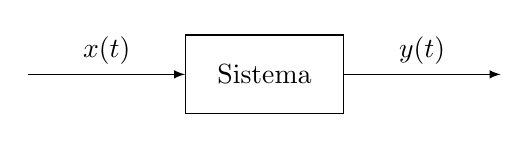
\begin{tikzpicture}[>=latex]
\node[draw, rectangle, minimum width=2cm, minimum height=1cm] (sys) at (0,0) {Sistema};
\draw[->] (-3,0) -- node[above] {$x(t)$} (sys.west);
\draw[->] (sys.east) -- node[above] {$y(t)$} (3,0);
\end{tikzpicture}
\end{center}

\vspace{0.3cm}

Um sistema é \textbf{Linear e Invariante no Tempo (LTI)} se possui duas propriedades:

\begin{enumerate}
\item \textbf{Linearidade:}
\[
x(t) = ax_1(t) + bx_2(t) \quad \Rightarrow \quad y(t) = ay_1(t) + by_2(t)
\]

\item \textbf{Invariância no tempo:}
\[
x(t - t_0) \quad \Rightarrow \quad y(t - t_0)
\]
\end{enumerate}

\textbf{Exemplos:} Filtros, amplificadores, canais de comunicação (sob condições ideais).

\end{frame}

% ============================================

\subsection{Resposta ao Impulso}

\begin{frame}{Resposta ao Impulso}

A \textbf{resposta ao impulso} $h(t)$ é a saída do sistema quando a entrada é $\delta(t)$:

\[
\delta(t) \quad \xrightarrow{\text{Sistema LTI}} \quad h(t)
\]

\textbf{Por que é importante?}

Qualquer sinal pode ser representado como soma de impulsos deslocados:
\[
x(t) = \int_{-\infty}^{\infty} x(\tau) \delta(t - \tau) d\tau
\]

Pela linearidade e invariância no tempo:
\[
y(t) = \int_{-\infty}^{\infty} x(\tau) h(t - \tau) d\tau = x(t) \conv h(t)
\]

\begin{block}{Relação Entrada-Saída no Tempo}
\[
\boxed{y(t) = x(t) \conv h(t)}
\]
\end{block}

\textbf{A resposta ao impulso caracteriza completamente um sistema LTI!}

\end{frame}

% ============================================

\subsection{Função de Transferência}

\begin{frame}{Função de Transferência (Resposta em Frequência)}

Aplicando a transformada de Fourier na relação $y(t) = x(t) \conv h(t)$:

\[
Y(\omega) = \FT{y(t)} = \FT{x(t) \conv h(t)}
\]

Pela propriedade de convolução:

\[
Y(\omega) = X(\omega) \cdot H(\omega)
\]

onde $H(\omega) = \FT{h(t)}$ é a \textbf{função de transferência} ou \textbf{resposta em frequência}.

\begin{block}{Relação Entrada-Saída na Frequência}
\[
\boxed{Y(\omega) = H(\omega) \cdot X(\omega)}
\]
\end{block}

\textbf{Vantagem:} Convolução no tempo $\rightarrow$ multiplicação na frequência!

A análise na frequência é muito mais simples.

\end{frame}

% ============================================

\begin{frame}{Interpretação da Função de Transferência}

\[
Y(\omega) = H(\omega) \cdot X(\omega)
\]

A função de transferência $H(\omega)$ é geralmente complexa:

\[
H(\omega) = |H(\omega)| e^{j\phi(\omega)}
\]

onde:
\begin{itemize}
\item $|H(\omega)|$: \textbf{ganho de magnitude} em cada frequência
\item $\phi(\omega) = \arg[H(\omega)]$: \textbf{mudança de fase} em cada frequência
\end{itemize}

\vspace{0.3cm}

\textbf{Efeito do sistema:}

\begin{itemize}
\item Cada componente de frequência de $X(\omega)$ é multiplicada por $|H(\omega)|$
\item A fase de cada componente é alterada por $\phi(\omega)$
\end{itemize}

\vspace{0.3cm}

\textbf{Aplicações:} Filtros selecionam/rejeitam certas frequências ajustando $|H(\omega)|$.

\end{frame}

% ============================================

\begin{frame}{Entrada Senoidal em Sistema LTI}

\textbf{Propriedade importante:} A resposta de um sistema LTI a uma entrada senoidal é também senoidal na mesma frequência.

Se $x(t) = A\cos(\omega_0 t + \theta)$, então:

\[
y(t) = A|H(\omega_0)| \cos(\omega_0 t + \theta + \phi(\omega_0))
\]

onde:
\begin{itemize}
\item Amplitude multiplicada por $|H(\omega_0)|$
\item Fase aumentada em $\phi(\omega_0)$
\item Frequência permanece $\omega_0$
\end{itemize}

\vspace{0.5cm}

\textbf{Demonstração:}

$x(t) = \Real\{Ae^{j(\omega_0 t + \theta)}\} = \Real\{Ae^{j\theta}e^{j\omega_0 t}\}$

Como $e^{j\omega_0 t} \xleftrightarrow{\ft} 2\pi\delta(\omega - \omega_0)$:

$y(t) = \Real\{Ae^{j\theta}H(\omega_0)e^{j\omega_0 t}\} = A|H(\omega_0)|\cos(\omega_0 t + \theta + \phi(\omega_0))$

\end{frame}

% ============================================

\subsection{Causalidade e Estabilidade}

\begin{frame}{Causalidade}

Um sistema é \textbf{causal} se a saída não depende de valores futuros da entrada:

\[
h(t) = 0 \quad \text{para} \quad t < 0
\]

\textbf{Significado físico:} Sistemas físicos reais são sempre causais (não podem "ver o futuro").

\vspace{0.3cm}

Para sistemas causais:
\[
y(t) = \int_{0}^{\infty} h(\tau) x(t - \tau) d\tau = \int_{-\infty}^{t} h(t - \tau) x(\tau) d\tau
\]

\vspace{0.3cm}

\textbf{Consequência na frequência:} A função de transferência $H(\omega)$ de um sistema causal satisfaz certas condições (critério de Paley-Wiener):

\[
\int_{-\infty}^{\infty} \frac{|\ln|H(\omega)||}{1 + \omega^2} d\omega < \infty
\]

Isso limita a rapidez com que $|H(\omega)|$ pode cair a zero.

\end{frame}

% ============================================

\begin{frame}{Estabilidade BIBO}

Um sistema é \textbf{BIBO estável} (Bounded Input, Bounded Output) se toda entrada limitada produz saída limitada.

\textbf{Critério de estabilidade:}

\[
\int_{-\infty}^{\infty} |h(t)| dt < \infty
\]

A resposta ao impulso deve ser absolutamente integrável.

\vspace{0.3cm}

\textbf{Na frequência:}

Para estabilidade BIBO, $H(\omega)$ deve existir e ser limitada:

\[
|H(\omega)| < \infty \quad \text{para todo} \quad \omega
\]

\vspace{0.3cm}

\textbf{Exemplos:}
\begin{itemize}
\item \textbf{Estável:} $h(t) = e^{-at}u(t)$ com $a > 0$
\item \textbf{Instável:} $h(t) = e^{at}u(t)$ com $a > 0$ (cresce exponencialmente)
\end{itemize}

\end{frame}

% ============================================

\subsection{Transmissão sem Distorção}

\begin{frame}{Condição para Transmissão sem Distorção}

\textbf{Objetivo:} Transmitir sinal sem alterar sua forma, apenas com ganho e atraso.

Desejamos:
\[
y(t) = K x(t - t_d)
\]

onde $K$ é um ganho constante e $t_d$ é um atraso fixo.

\vspace{0.3cm}

\textbf{Condição na frequência:}

Aplicando a transformada de Fourier:

\[
Y(\omega) = K X(\omega) e^{-j\omega t_d}
\]

Como $Y(\omega) = H(\omega)X(\omega)$:

\[
H(\omega)X(\omega) = K X(\omega) e^{-j\omega t_d}
\]

\end{frame}

% ============================================

\begin{frame}{Função de Transferência Ideal}

Para transmissão sem distorção:

\begin{block}{Condição de Transmissão sem Distorção}
\[
\boxed{H(\omega) = K e^{-j\omega t_d}}
\]
\end{block}

Isto significa:
\begin{itemize}
\item \textbf{Magnitude constante:} $|H(\omega)| = K$ para todas as frequências
\item \textbf{Fase linear:} $\phi(\omega) = -\omega t_d$ (proporcional a $\omega$)
\end{itemize}

\vspace{0.3cm}

\textbf{Interpretação física:}
\begin{itemize}
\item Todas as componentes de frequência têm mesmo ganho
\item Todas as componentes sofrem mesmo atraso $t_d$
\item A forma de onda é preservada
\end{itemize}

\vspace{0.3cm}

\textbf{Problema:} Sistemas reais não podem ter $|H(\omega)|$ constante para todo $\omega$ e serem causais simultaneamente!

\end{frame}

% ============================================

\subsection{Distorção em Sistemas}

\begin{frame}{Tipos de Distorção}

Quando $H(\omega) \neq K e^{-j\omega t_d}$, ocorre distorção:

\begin{enumerate}
\item \textbf{Distorção de Amplitude:}
   \begin{itemize}
   \item $|H(\omega)|$ não é constante
   \item Algumas frequências são amplificadas/atenuadas mais que outras
   \item Altera o formato do sinal
   \end{itemize}

\item \textbf{Distorção de Fase:}
   \begin{itemize}
   \item $\phi(\omega)$ não é linear com $\omega$
   \item Diferentes frequências sofrem atrasos diferentes
   \item Componentes chegam "fora de sincronia"
   \end{itemize}
\end{enumerate}

\vspace{0.3cm}

\textbf{Ambos os tipos degradam o sinal!}

Em sistemas práticos, busca-se minimizar distorção na banda de interesse.

\end{frame}

% ============================================

\begin{frame}{Atraso de Grupo}

O \textbf{atraso de grupo} quantifica o atraso de um "envelope" do sinal:

\[
\tau_g(\omega) = -\frac{d\phi(\omega)}{d\omega}
\]

\textbf{Interpretação:}
\begin{itemize}
\item Se $\phi(\omega) = -\omega t_d$ (linear), então $\tau_g = t_d$ (constante)
\item Se $\tau_g(\omega)$ varia, diferentes frequências têm atrasos diferentes
\item Causa distorção de fase
\end{itemize}

\vspace{0.3cm}

\textbf{Para transmissão sem distorção de fase:}

\[
\tau_g(\omega) = \text{constante}
\]

\vspace{0.3cm}

\textbf{Aplicação:} Importante em sinais modulados e pulsos digitais, onde o envelope carrega informação.

\end{frame}

% ============================================

\subsection{Largura de Banda}

\begin{frame}{Largura de Banda de Sistemas}

A \textbf{largura de banda} de um sistema mede a faixa de frequências que o sistema transmite eficientemente.

\textbf{Definições comuns:}

\begin{enumerate}
\item \textbf{Largura de banda de 3 dB:}
   \[
   |H(\omega)| \geq \frac{|H(\omega_{\max})|}{\sqrt{2}}
   \]
   Frequências onde o ganho cai no máximo 3 dB (metade da potência).

\item \textbf{Largura de banda de ruído:}
   \[
   B_n = \frac{1}{|H(\omega_{\max})|^2} \int_{-\infty}^{\infty} |H(\omega)|^2 d\omega
   \]

\item \textbf{Largura de banda absoluta:}
   
   Faixa onde $|H(\omega)| > 0$ (pode ser infinita).
\end{enumerate}

\textbf{Princípio:} Sistemas de banda limitada introduzem distorção em sinais de banda larga.

\end{frame}

% ============================================

\subsection{Exemplos de Sistemas LTI}

\begin{frame}{Exemplo 1: Filtro RC Passa-Baixas}

Circuito RC série com saída no capacitor:

\begin{center}
\begin{tikzpicture}[>=latex, american voltages]
% Entrada
\draw (0,0) -- (0,2);
\draw[<-] (0,2.2) -- (0,2.5) node[above] {$x(t)$};
% Resistor
\draw (0,2) -- (1,2);
\draw (1,1.5) rectangle (2,2.5) node[midway] {$R$};
\draw (2,2) -- (3,2);
% Capacitor
\draw (3,2) -- (3,1.5);
\draw (2.7,1.5) -- (3.3,1.5);
\draw (2.7,1) -- (3.3,1);
\draw (3,1) -- (3,0);
\node[right] at (3.3,1.25) {$C$};
% Terra
\draw (0,0) -- (3,0);
\draw (1.5,0) -- (1.5,-0.3) node[ground] {};
% Saída
\draw (3,1.25) -- (4,1.25);
\draw[->] (4,1.25) -- (4,1.75) node[above] {$y(t)$};
\end{tikzpicture}
\end{center}

\textbf{Equação diferencial:}
\[
RC\frac{dy(t)}{dt} + y(t) = x(t)
\]

\textbf{Transformada de Fourier:}
\[
RC \cdot j\omega Y(\omega) + Y(\omega) = X(\omega)
\]

\[
Y(\omega)[1 + j\omega RC] = X(\omega)
\]

\end{frame}

% ============================================

\begin{frame}{Exemplo 1: Função de Transferência do Filtro RC}

\[
H(\omega) = \frac{Y(\omega)}{X(\omega)} = \frac{1}{1 + j\omega RC}
\]

Definindo a \textbf{frequência de corte}: $\omega_c = 1/(RC)$

\[
H(\omega) = \frac{1}{1 + j\omega/\omega_c} = \frac{\omega_c}{\omega_c + j\omega}
\]

\textbf{Magnitude:}
\[
|H(\omega)| = \frac{1}{\sqrt{1 + (\omega/\omega_c)^2}}
\]

\textbf{Fase:}
\[
\phi(\omega) = -\arctan(\omega/\omega_c)
\]

\textbf{Características:}
\begin{itemize}
\item Em $\omega = 0$: $|H(0)| = 1$ (DC passa)
\item Em $\omega = \omega_c$: $|H(\omega_c)| = 1/\sqrt{2}$ (ponto de 3 dB)
\item Em $\omega \to \infty$: $|H(\omega)| \to 0$ (altas frequências atenuadas)
\end{itemize}

\end{frame}

% ============================================

\begin{frame}{Exemplo 1: Resposta em Frequência do Filtro RC}

\begin{center}
\includegraphics[width=\figFull, height=0.68\textheight, keepaspectratio]{figures/cap3/exponential_fourier}
\end{center}

\vspace{-0.3cm}
\begin{itemize}
\item A magnitude $|H(\omega)|$ é uma Lorentziana: máxima em DC, cai $-3\,\text{dB}$ em $\omega_c$
\item A fase $\phi(\omega) = -\arctan(\omega/\omega_c)$ é \textbf{não-linear} $\Rightarrow$ distorção de fase
\end{itemize}

\end{frame}

% ============================================

\begin{frame}{Exemplo 1: Resposta ao Impulso do Filtro RC}

A resposta ao impulso é a transformada inversa de $H(\omega)$:

\[
H(\omega) = \frac{\omega_c}{\omega_c + j\omega}
\]

Reconhecemos: $\frac{1}{a + j\omega} \xleftrightarrow{\ft} e^{-at}u(t)$

Portanto:

\[
h(t) = \omega_c e^{-\omega_c t} u(t) = \frac{1}{RC} e^{-t/(RC)} u(t)
\]

\textbf{Propriedades:}
\begin{itemize}
\item Causal: $h(t) = 0$ para $t < 0$
\item Estável: $\int_0^{\infty} h(t)dt = 1 < \infty$
\item Decai exponencialmente com constante de tempo $\tau = RC$
\end{itemize}

\textbf{Interpretação física:} O capacitor "suaviza" mudanças rápidas (altas frequências).

\end{frame}

% ============================================

\begin{frame}{Exemplo 2: Filtro Ideal Passa-Baixas}

Um filtro passa-baixas ideal tem função de transferência:

\[
H(\omega) = \begin{cases}
1 & |\omega| \leq \omega_c \\
0 & |\omega| > \omega_c
\end{cases} = \rect\left(\frac{\omega}{2\omega_c}\right)
\]

\textbf{Resposta ao impulso:}

Pela dualidade, sabemos que $\rect(t/\tau) \xleftrightarrow{\ft} \tau\sinc(\omega\tau/2\pi)$

Aplicando dualidade inversa:

\[
h(t) = \frac{\omega_c}{\pi} \sinc\left(\frac{\omega_c t}{\pi}\right) = \frac{\sin(\omega_c t)}{\pi t}
\]

\textbf{Problema:} $h(t) \neq 0$ para $t < 0$ $\rightarrow$ \textbf{não-causal}!

Filtro ideal passa-baixas é fisicamente irrealizável.

\end{frame}

% ============================================

\begin{frame}{Exemplo 2: Por que o Filtro Ideal é Irrealizável?}

\[
h(t) = \frac{\sin(\omega_c t)}{\pi t}
\]

\textbf{Problemas:}

\begin{enumerate}
\item \textbf{Não-causalidade:}
   \begin{itemize}
   \item $h(t) \neq 0$ para todo $t < 0$
   \item Sistema responde antes do impulso ser aplicado!
   \item Violação da causalidade física
   \end{itemize}

\item \textbf{Duração infinita:}
   \begin{itemize}
   \item $h(t)$ não decai a zero em tempo finito
   \item Oscila indefinidamente como $1/t$
   \item Impossível implementar exatamente
   \end{itemize}
\end{enumerate}

\vspace{0.3cm}

\textbf{Solução prática:} Usar filtros aproximados (Butterworth, Chebyshev) que são causais e aproximam o comportamento ideal.

\end{frame}

% ============================================

\begin{frame}{Resumo da Seção 3.4}

\textbf{Conceitos fundamentais de sistemas LTI:}

\begin{itemize}
\item \textbf{No tempo:} $y(t) = x(t) \conv h(t)$
\item \textbf{Na frequência:} $Y(\omega) = H(\omega) X(\omega)$
\item Análise na frequência simplifica cálculos!
\end{itemize}

\vspace{0.3cm}

\textbf{Propriedades importantes:}

\begin{itemize}
\item Causalidade: $h(t) = 0$ para $t < 0$
\item Estabilidade BIBO: $\int|h(t)|dt < \infty$
\item Transmissão sem distorção: $H(\omega) = Ke^{-j\omega t_d}$
\end{itemize}

\vspace{0.3cm}

\textbf{Tipos de distorção:}

\begin{itemize}
\item Amplitude: $|H(\omega)|$ não constante
\item Fase: $\phi(\omega)$ não linear
\end{itemize}

\textbf{Próximo:} Filtros ideais versus práticos.

\end{frame}


% ============================================
% SEÇÃO 3.5: FILTROS IDEAIS VERSUS PRÁTICOS
% ============================================
\section{Filtros Ideais versus Práticos}
% ============================================
% SEÇÃO 3.5: FILTROS IDEAIS VERSUS PRÁTICOS
% ============================================

\subsection{Filtros Ideais}

\begin{frame}{Tipos de Filtros Ideais: Passa-Baixas e Passa-Altas}

\begin{columns}[T]
\column{0.48\textwidth}
\textbf{Passa-Baixas (LP):}
\[
H_{LP}(\omega) = \begin{cases}
1, & |\omega| \leq \omega_c \\
0, & |\omega| > \omega_c
\end{cases}
\]
\vspace{-0.2cm}
\begin{center}
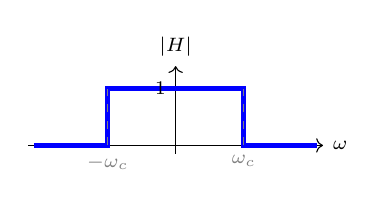
\begin{tikzpicture}[scale=0.72]
\draw[->] (-2.6,0) -- (2.6,0) node[right,font=\scriptsize] {$\omega$};
\draw[->] (0,-0.15) -- (0,1.4) node[above,font=\scriptsize] {$|H|$};
\draw[line width=1.8pt,blue] (-2.5,0) -- (-1.2,0) -- (-1.2,1) -- (1.2,1) -- (1.2,0) -- (2.5,0);
\draw[dashed,gray] (-1.2,0) node[below,font=\scriptsize] {$-\omega_c$} -- (-1.2,1);
\draw[dashed,gray] (1.2,0) node[below,font=\scriptsize] {$\omega_c$} -- (1.2,1);
\node[left,font=\scriptsize] at (0,1) {$1$};
\end{tikzpicture}
\end{center}
Passa frequências \textbf{abaixo} de $\omega_c$.

\column{0.48\textwidth}
\textbf{Passa-Altas (HP):}
\[
H_{HP}(\omega) = \begin{cases}
0, & |\omega| < \omega_c \\
1, & |\omega| \geq \omega_c
\end{cases}
\]
\vspace{-0.2cm}
\begin{center}
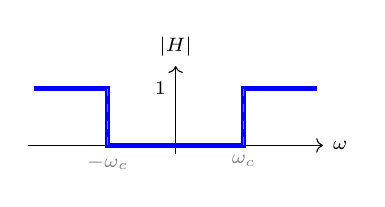
\begin{tikzpicture}[scale=0.72]
\draw[->] (-2.6,0) -- (2.6,0) node[right,font=\scriptsize] {$\omega$};
\draw[->] (0,-0.15) -- (0,1.4) node[above,font=\scriptsize] {$|H|$};
\draw[line width=1.8pt,blue] (-2.5,1) -- (-1.2,1) -- (-1.2,0) -- (1.2,0) -- (1.2,1) -- (2.5,1);
\draw[dashed,gray] (-1.2,0) node[below,font=\scriptsize] {$-\omega_c$} -- (-1.2,1);
\draw[dashed,gray] (1.2,0) node[below,font=\scriptsize] {$\omega_c$} -- (1.2,1);
\node[left,font=\scriptsize] at (0,1) {$1$};
\end{tikzpicture}
\end{center}
Passa frequências \textbf{acima} de $\omega_c$.
\end{columns}

\end{frame}

% ============================================

\begin{frame}{Tipos de Filtros Ideais: Passa-Faixas e Rejeita-Faixas}

\begin{columns}[T]
\column{0.48\textwidth}
\textbf{Passa-Faixas (BP):}
\[
H_{BP}(\omega) = \begin{cases}
1, & \omega_1 \!\leq\! |\omega| \!\leq\! \omega_2 \\
0, & \text{caso contrário}
\end{cases}
\]
\vspace{-0.2cm}
\begin{center}
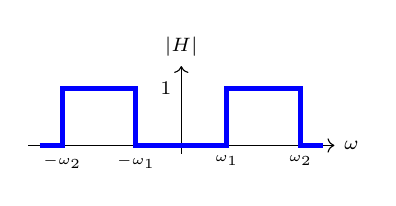
\begin{tikzpicture}[scale=0.72]
\draw[->] (-2.7,0) -- (2.7,0) node[right,font=\scriptsize] {$\omega$};
\draw[->] (0,-0.15) -- (0,1.4) node[above,font=\scriptsize] {$|H|$};
\draw[line width=1.8pt,blue]
  (-2.5,0) -- (-2.1,0) -- (-2.1,1) -- (-0.8,1) -- (-0.8,0)
  -- (0.8,0) -- (0.8,1) -- (2.1,1) -- (2.1,0) -- (2.5,0);
\node[below,font=\tiny] at (-2.1,0) {$-\omega_2$};
\node[below,font=\tiny] at (-0.8,0) {$-\omega_1$};
\node[below,font=\tiny] at (0.8,0) {$\omega_1$};
\node[below,font=\tiny] at (2.1,0) {$\omega_2$};
\node[left,font=\scriptsize] at (0,1) {$1$};
\end{tikzpicture}
\end{center}
Passa uma \textbf{faixa} entre $\omega_1$ e $\omega_2$.

\column{0.48\textwidth}
\textbf{Rejeita-Faixas (BS):}
\[
H_{BS}(\omega) = \begin{cases}
0, & \omega_1 \!<\! |\omega| \!<\! \omega_2 \\
1, & \text{caso contrário}
\end{cases}
\]
\vspace{-0.2cm}
\begin{center}
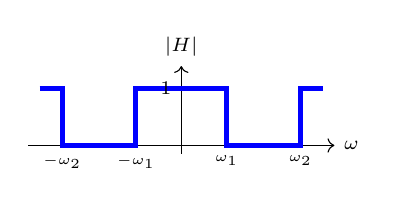
\begin{tikzpicture}[scale=0.72]
\draw[->] (-2.7,0) -- (2.7,0) node[right,font=\scriptsize] {$\omega$};
\draw[->] (0,-0.15) -- (0,1.4) node[above,font=\scriptsize] {$|H|$};
\draw[line width=1.8pt,blue]
  (-2.5,1) -- (-2.1,1) -- (-2.1,0) -- (-0.8,0) -- (-0.8,1)
  -- (0.8,1) -- (0.8,0) -- (2.1,0) -- (2.1,1) -- (2.5,1);
\node[below,font=\tiny] at (-2.1,0) {$-\omega_2$};
\node[below,font=\tiny] at (-0.8,0) {$-\omega_1$};
\node[below,font=\tiny] at (0.8,0) {$\omega_1$};
\node[below,font=\tiny] at (2.1,0) {$\omega_2$};
\node[left,font=\scriptsize] at (0,1) {$1$};
\end{tikzpicture}
\end{center}
\textbf{Bloqueia} uma faixa entre $\omega_1$ e $\omega_2$.
\end{columns}

\end{frame}

% ============================================

\begin{frame}{Características de Filtros Ideais}

\textbf{Propriedades dos filtros ideais:}

\begin{itemize}
\item \textbf{Banda passante:} $|H(\omega)| = 1$ (ganho unitário, sem atenuação)
\item \textbf{Banda de rejeição:} $|H(\omega)| = 0$ (atenuação infinita)
\item \textbf{Banda de transição:} Largura zero (mudança instantânea)
\item \textbf{Fase linear:} $\phi(\omega) = -\omega t_d$ na banda passante
\item \textbf{Seletividade perfeita:} Separa exatamente as frequências desejadas
\end{itemize}

\vspace{0.5cm}

\textbf{Aplicações teóricas:}
\begin{itemize}
\item Análise de sistemas de comunicação
\item Determinação de limites de desempenho
\item Referência para comparação com filtros reais
\end{itemize}

\vspace{0.3cm}

\textbf{Problema:} Filtros ideais são \textbf{fisicamente irrealizáveis}!

\end{frame}

% ============================================

\subsection{Problema da Causalidade}

\begin{frame}{Resposta ao Impulso do Filtro Passa-Baixas Ideal}

Já vimos que para $H_{LP}(\omega) = \rect(\omega/2\omega_c)$:

\[
h_{LP}(t) = \frac{\omega_c}{\pi} \sinc\left(\frac{\omega_c t}{\pi}\right) = \frac{\sin(\omega_c t)}{\pi t}
\]

\textbf{Análise da resposta:}

\begin{itemize}
\item Máximo em $t = 0$: $h_{LP}(0) = \omega_c/\pi$
\item Zeros em $t = \pm n\pi/\omega_c$ para $n = 1, 2, 3, ...$
\item \textbf{Existe para todo} $t \in (-\infty, \infty)$
\item Decai como $1/t$ (lentamente)
\end{itemize}

\vspace{0.3cm}

\textbf{Problema crítico:}

\[
h_{LP}(t) \neq 0 \quad \text{para} \quad t < 0
\]

O filtro responde \textbf{antes} do impulso ser aplicado!

\textbf{Conclusão:} Viola causalidade $\rightarrow$ fisicamente impossível.

\end{frame}

% ============================================

\begin{frame}{Critério de Paley-Wiener}

\textbf{Teorema (Paley-Wiener):}

Um filtro com função de transferência $H(\omega)$ é causalmente realizável se e somente se:

\[
\int_{-\infty}^{\infty} \frac{|\ln |H(\omega)||}{1 + \omega^2} d\omega < \infty
\]

\textbf{Consequências práticas:}

\begin{enumerate}
\item $|H(\omega)|$ não pode ser zero em nenhuma banda finita de frequências
\item A transição de banda passante para banda de rejeição deve ser gradual
\item $|H(\omega)|$ não pode cair a zero "rápido demais"
\end{enumerate}

\vspace{0.3cm}

\textbf{Para filtro ideal passa-baixas:}

$H(\omega) = 0$ para $|\omega| > \omega_c$ $\rightarrow$ $\ln|H(\omega)| = -\infty$

A integral diverge $\rightarrow$ \textbf{não satisfaz o critério} $\rightarrow$ não-causal.

\end{frame}

% ============================================

\begin{frame}{Aproximação de Filtros Ideais}

Como filtros ideais são irrealizáveis, usamos \textbf{aproximações causais}:

\textbf{Estratégias de aproximação:}

\begin{enumerate}
\item \textbf{Permitir banda de transição finita:}
   
   Mudança gradual entre passante e rejeição

\item \textbf{Permitir ondulação (ripple):}
   
   $|H(\omega)|$ não perfeitamente constante

\item \textbf{Atenuação finita na banda de rejeição:}
   
   $|H(\omega)| \neq 0$, mas muito pequeno

\item \textbf{Fase não perfeitamente linear:}
   
   Alguma distorção de fase aceitável
\end{enumerate}

\vspace{0.3cm}

\textbf{Compromissos inevitáveis:}

Não podemos ter simultaneamente: seletividade perfeita, causalidade, fase linear e complexidade finita.

\end{frame}

% ============================================

\subsection{Filtros Práticos}

\begin{frame}{Especificações de Filtros Práticos}

Um filtro prático passa-baixas é especificado por:

\begin{itemize}
\item \textbf{Banda passante:} $0 \leq \omega \leq \omega_p$
  \begin{itemize}
  \item Variação permitida: $1 - \delta_1 \leq |H(\omega)| \leq 1 + \delta_1$
  \item Ripple típico: $\delta_1 = 0.1$ (ondulação de 1 dB)
  \end{itemize}

\item \textbf{Banda de transição:} $\omega_p < \omega < \omega_s$
  \begin{itemize}
  \item Região onde $|H(\omega)|$ muda de passante para rejeição
  \item Quanto mais estreita, mais complexo o filtro
  \end{itemize}

\item \textbf{Banda de rejeição:} $\omega \geq \omega_s$
  \begin{itemize}
  \item Atenuação mínima: $|H(\omega)| \leq \delta_2$
  \item Atenuação típica: $\delta_2 = 0.01$ (40 dB)
  \end{itemize}
\end{itemize}

\vspace{0.3cm}

\textbf{Parâmetros de projeto:}
\begin{itemize}
\item Frequência de corte passante: $\omega_p$ ou $f_p$
\item Frequência de corte de rejeição: $\omega_s$ ou $f_s$
\item Ordem do filtro: $n$ (número de polos)
\end{itemize}

\end{frame}

% ============================================

\begin{frame}{Filtro de Butterworth}

O \textbf{filtro de Butterworth} maximiza a planura na banda passante.

\textbf{Função de transferência:}

\[
|H(\omega)|^2 = \frac{1}{1 + (\omega/\omega_c)^{2n}}
\]

onde $n$ é a ordem do filtro e $\omega_c$ é a frequência de corte de 3 dB.

\textbf{Propriedades:}

\begin{itemize}
\item Em $\omega = 0$: $|H(0)| = 1$ (ganho unitário em DC)
\item Em $\omega = \omega_c$: $|H(\omega_c)| = 1/\sqrt{2} \approx 0.707$ (-3 dB)
\item \textbf{Resposta maximally flat:} Primeiras $2n-1$ derivadas são zero em $\omega = 0$
\item Decaimento: $20n$ dB/década para $\omega \gg \omega_c$
\item Sem ondulação na banda passante ou de rejeição
\end{itemize}

\vspace{0.3cm}

\textbf{Características de fase:}
\begin{itemize}
\item Fase não-linear (especialmente próximo a $\omega_c$)
\item Distorção de fase presente
\end{itemize}

\end{frame}

% ============================================

\begin{frame}{Butterworth: Efeito da Ordem}

\[
|H(\omega)|^2 = \frac{1}{1 + (\omega/\omega_c)^{2n}}
\]

\textbf{Análise por ordem:}

\begin{itemize}
\item \textbf{$n = 1$:} Filtro RC simples, decaimento 20 dB/década
\item \textbf{$n = 2$:} Decaimento 40 dB/década, transição mais rápida
\item \textbf{$n \to \infty$:} Aproxima-se do filtro ideal (mas sempre causal)
\end{itemize}

\vspace{0.3cm}

\textbf{Relação ordem-transição:}

Para especificações dadas ($\omega_p$, $\omega_s$, $\delta_1$, $\delta_2$), a ordem necessária é:

\[
n \geq \frac{\log\left[\frac{(1/\delta_2)^2 - 1}{(1/\delta_1)^2 - 1}\right]}{2\log(\omega_s/\omega_p)}
\]

\vspace{0.3cm}

\textbf{Compromisso:} Maior ordem $\rightarrow$ melhor seletividade, mas maior complexidade e atraso.

\end{frame}

% ============================================

\begin{frame}{Filtro de Chebyshev Tipo I}

O \textbf{filtro de Chebyshev Tipo I} permite ondulação na banda passante para obter transição mais rápida.

\textbf{Função de transferência:}

\[
|H(\omega)|^2 = \frac{1}{1 + \epsilon^2 T_n^2(\omega/\omega_c)}
\]

onde:
\begin{itemize}
\item $T_n(x)$ é o polinômio de Chebyshev de ordem $n$
\item $\epsilon$ controla a ondulação na banda passante
\end{itemize}

\textbf{Propriedades:}

\begin{itemize}
\item \textbf{Ondulação equi-ripple} na banda passante: oscila entre 1 e $1/\sqrt{1+\epsilon^2}$
\item Banda de rejeição monótona (sem ondulação)
\item Decaimento mais rápido que Butterworth de mesma ordem
\item Para mesma seletividade, requer ordem menor que Butterworth
\end{itemize}

\textbf{Desvantagem:} Ondulação pode ser indesejável em algumas aplicações.

\end{frame}

% ============================================

\begin{frame}{Filtro de Chebyshev Tipo II (Inverso)}

O \textbf{filtro de Chebyshev Tipo II} permite ondulação na banda de rejeição.

\textbf{Características:}

\begin{itemize}
\item Banda passante monótona (sem ondulação)
\item Ondulação equi-ripple na banda de rejeição
\item Transição mais gradual que Tipo I
\item Zeros de transmissão na banda de rejeição
\end{itemize}

\vspace{0.5cm}

\textbf{Comparação dos tipos:}

\begin{center}
\small
\begin{tabular}{|l|c|c|}
\hline
\textbf{Característica} & \textbf{Tipo I} & \textbf{Tipo II} \\
\hline
Banda passante & Ondulação & Monótona \\
\hline
Banda de rejeição & Monótona & Ondulação \\
\hline
Transição & Mais rápida & Mais gradual \\
\hline
\end{tabular}
\end{center}

\end{frame}

% ============================================

\begin{frame}{Filtro de Bessel (Thomson)}

O \textbf{filtro de Bessel} maximiza a linearidade da fase.

\textbf{Objetivo:} Minimizar distorção de fase, ideal para pulsos.

\textbf{Propriedades:}

\begin{itemize}
\item \textbf{Fase aproximadamente linear} na banda passante
\item \textbf{Atraso de grupo aproximadamente constante:} $\tau_g(\omega) \approx \tau_0$
\item Resposta ao degrau com mínimo overshoot e ringing
\item Preserva melhor a forma de pulsos
\end{itemize}

\vspace{0.3cm}

\textbf{Desvantagem:}

\begin{itemize}
\item Seletividade pior que Butterworth ou Chebyshev
\item Para mesmas especificações, requer ordem maior
\item Banda de transição mais larga
\end{itemize}

\vspace{0.3cm}

\textbf{Aplicação ideal:} Transmissão de dados digitais onde preservar formato do pulso é crítico.

\end{frame}

% ============================================

\begin{frame}{Filtro Elíptico (Cauer)}

O \textbf{filtro elíptico} permite ondulação tanto na banda passante quanto na de rejeição.

\textbf{Características:}

\begin{itemize}
\item Ondulação equi-ripple em \textbf{ambas} as bandas
\item \textbf{Transição mais rápida} entre todas as aproximações
\item Para especificações dadas, requer a \textbf{menor ordem}
\item Zeros de transmissão na banda de rejeição e no eixo $j\omega$
\end{itemize}

\vspace{0.3cm}

\textbf{Função de transferência:}

\[
|H(\omega)|^2 = \frac{1}{1 + \epsilon^2 R_n^2(\omega/\omega_c)}
\]

onde $R_n$ é uma função racional (razão de polinômios).

\vspace{0.3cm}

\textbf{Aplicação:} Quando a ordem mínima é crítica (custo, consumo de energia).

\textbf{Desvantagem:} Fase muito não-linear, maior distorção de fase.

\end{frame}

% ============================================

\begin{frame}{Comparação Visual: Filtros Práticos de Ordem 4}

\begin{center}
\includegraphics[width=\figFull, height=0.72\textheight, keepaspectratio]{figures/cap3/filters_comparison}
\end{center}

\vspace{-0.3cm}
\begin{block}{Observação}
Butterworth: passante plana, sem ondulação. \quad Chebyshev: transição mais rápida. \quad Bessel: fase mais linear.
\end{block}

\end{frame}

% ============================================

\begin{frame}{Comparação de Aproximações de Filtros}

\textbf{Para mesma ordem $n$ e frequência de corte $\omega_c$:}

\begin{center}
\small
\begin{tabular}{|l|c|c|c|c|}
\hline
\textbf{Característica} & \textbf{Butter.} & \textbf{Cheby I} & \textbf{Bessel} & \textbf{Elíptico} \\
\hline
Planura passante & Boa & Ripple & Melhor & Ripple \\
\hline
Seletividade & Média & Boa & Fraca & Melhor \\
\hline
Fase linear & Média & Fraca & Melhor & Fraca \\
\hline
Ordem necessária & Média & Baixa & Alta & Mínima \\
\hline
Complexidade & Média & Média & Baixa & Alta \\
\hline
\end{tabular}
\end{center}

\vspace{0.5cm}

\textbf{Escolha do filtro depende da aplicação:}

\begin{itemize}
\item \textbf{Áudio:} Butterworth ou Bessel (fase linear)
\item \textbf{Comunicação digital:} Bessel (preserva pulsos)
\item \textbf{Separação espectral:} Chebyshev ou Elíptico (seletividade)
\item \textbf{Geral:} Butterworth (compromisso balanceado)
\end{itemize}

\end{frame}

% ============================================

\subsection{Relação Ordem-Desempenho}

\begin{frame}{Determinação da Ordem do Filtro}

\textbf{Problema:} Dadas especificações, determinar a ordem mínima necessária.

\textbf{Para filtro Butterworth passa-baixas:}

Especificações:
\begin{itemize}
\item Passante: $|H(\omega)| \geq 1 - \delta_1$ para $\omega \leq \omega_p$
\item Rejeição: $|H(\omega)| \leq \delta_2$ para $\omega \geq \omega_s$
\end{itemize}

A ordem necessária é:

\[
n = \left\lceil \frac{\log\left[\frac{(1/\delta_2)^2 - 1}{(1/\delta_1)^2 - 1}\right]}{2\log(\omega_s/\omega_p)} \right\rceil
\]

onde $\lceil \cdot \rceil$ é a função teto (arredondamento para cima).

\vspace{0.3cm}

\textbf{Simplificação prática:} Para $\delta_1, \delta_2 \ll 1$:

\[
n \approx \frac{\log(1/\delta_2) - \log(1/\delta_1)}{2\log(\omega_s/\omega_p)}
\]

\end{frame}

% ============================================

\begin{frame}{Exemplo: Projeto de Filtro Butterworth}

\textbf{Especificações:}

\begin{itemize}
\item Frequência de passante: $f_p = 1$ kHz
\item Frequência de rejeição: $f_s = 3$ kHz
\item Ondulação na passante: máx 1 dB ($\delta_1 = 0.1$, i.e., $|H| \geq 0.891$)
\item Atenuação na rejeição: mín 30 dB ($\delta_2 = 0.0316$, i.e., $|H| \leq 0.0316$)
\end{itemize}

\textbf{Cálculo da ordem:}

\[
n = \left\lceil \frac{\log[(1/0.0316)^2 - 1] - \log[(1/0.891)^2 - 1]}{2\log(3000/1000)} \right\rceil
\]

\[
= \left\lceil \frac{\log(1001) - \log(0.259)}{2\log(3)} \right\rceil = \left\lceil \frac{3.00 - (-0.587)}{2 \times 0.477} \right\rceil
\]

\[
= \left\lceil \frac{3.587}{0.954} \right\rceil = \lceil 3.76 \rceil = 4
\]

\textbf{Resultado:} Necessário filtro Butterworth de ordem 4.

\end{frame}

% ============================================

\begin{frame}{Implementação de Filtros}

\textbf{Formas de implementação:}

\begin{enumerate}
\item \textbf{Filtros analógicos (tempo contínuo):}
   \begin{itemize}
   \item Resistores, capacitores, indutores, amplificadores operacionais
   \item Implementação direta da função de transferência $H(s)$
   \item Limitados por componentes físicos
   \end{itemize}

\item \textbf{Filtros digitais (tempo discreto):}
   \begin{itemize}
   \item Algoritmos implementados em DSP, FPGA, software
   \item Versão discreta após conversão A/D
   \item Maior flexibilidade, estabilidade, reprodutibilidade
   \end{itemize}
\end{enumerate}

\vspace{0.3cm}

\textbf{Estruturas de implementação:}

\begin{itemize}
\item Cascata (série de seções de 2ª ordem)
\item Paralela (soma de seções)
\item Ladder (escada), para filtros passivos
\end{itemize}

\end{frame}

% ============================================

\begin{frame}{Resumo da Seção 3.5}

\textbf{Filtros ideais:}

\begin{itemize}
\item Seletividade perfeita, mas fisicamente irrealizáveis
\item Violam causalidade (critério de Paley-Wiener)
\item Servem como referência teórica
\end{itemize}

\vspace{0.3cm}

\textbf{Filtros práticos (aproximações causais):}

\begin{itemize}
\item \textbf{Butterworth:} Resposta plana, compromisso geral
\item \textbf{Chebyshev:} Ripple para maior seletividade
\item \textbf{Bessel:} Fase linear, preserva pulsos
\item \textbf{Elíptico:} Ordem mínima, máxima seletividade
\end{itemize}

\vspace{0.3cm}

\textbf{Compromissos inevitáveis:}

Seletividade $\leftrightarrow$ Fase linear $\leftrightarrow$ Complexidade

\textbf{Projeto:} Escolher aproximação e ordem baseado em especificações e aplicação.

\end{frame}


% ============================================
% SEÇÃO 3.6: DISTORÇÃO DE SINAL EM CANAIS
% ============================================
\section{Distorção de Sinal em Canais de Comunicação}
% ============================================
% SEÇÃO 3.6: DISTORÇÃO DE SINAL EM CANAIS
% ============================================

\subsection{Modelo de Canal de Comunicação}

\begin{frame}{Canal como Sistema LTI}

Em um sistema de comunicação, o canal pode ser modelado como um sistema LTI:

\begin{center}
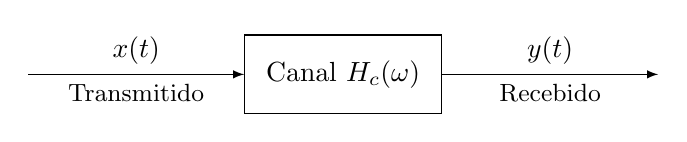
\begin{tikzpicture}[>=latex]
\node[draw, rectangle, minimum width=2.5cm, minimum height=1cm] (canal) at (0,0) {Canal $H_c(\omega)$};
\draw[->] (-4,0) -- node[above] {$x(t)$} node[below] {\small Transmitido} (canal.west);
\draw[->] (canal.east) -- node[above] {$y(t)$} node[below] {\small Recebido} (4,0);
\end{tikzpicture}
\end{center}

\textbf{Relação entrada-saída:}

No tempo: $y(t) = x(t) \conv h_c(t)$

Na frequência: $Y(\omega) = H_c(\omega) X(\omega)$

\vspace{0.3cm}

\textbf{Canal ideal:}
\[
H_c(\omega) = K e^{-j\omega t_d}
\]

Apenas amplifica e atrasa o sinal, sem alterar sua forma.

\vspace{0.3cm}

\textbf{Canal real:} $H_c(\omega)$ tem $|H_c(\omega)|$ e $\phi_c(\omega)$ variáveis, causando distorção.

\end{frame}

% ============================================

\subsection{Tipos de Distorção}

\begin{frame}{Distorção de Amplitude}

\textbf{Causa:} $|H_c(\omega)|$ não é constante na banda do sinal.

\textbf{Efeito:}

Diferentes componentes de frequência são amplificadas/atenuadas diferentemente:

\[
|Y(\omega)| = |H_c(\omega)| \cdot |X(\omega)|
\]

\textbf{Consequências práticas:}

\begin{itemize}
\item Alteração do formato da forma de onda
\item Componentes importantes podem ser atenuadas
\item Interferência entre símbolos (ISI) em comunicação digital
\item Degradação da relação sinal-ruído
\end{itemize}

\textbf{Exemplo típico:}

Canal telefônico: atenuação aumenta com frequência (efeito de cabo)

\[
|H_c(\omega)| \approx e^{-\alpha \omega}
\]

Altas frequências sofrem maior atenuação que baixas frequências.

\end{frame}

% ============================================

\begin{frame}{Exemplo: Distorção de Amplitude}

\textbf{Situação:} Pulso quadrado transmitido através de canal passa-baixas.

Pulso quadrado contém harmônicas ímpares: $\omega_0, 3\omega_0, 5\omega_0, ...$

\textbf{Canal com resposta:}
\[
|H_c(\omega)| = \begin{cases}
1 & |\omega| \leq 3\omega_0 \\
0.5 & 3\omega_0 < |\omega| \leq 5\omega_0 \\
0.1 & |\omega| > 5\omega_0
\end{cases}
\]

\textbf{Efeito na recepção:}

\begin{itemize}
\item Fundamental ($\omega_0$): passa sem alteração
\item 3ª harmônica ($3\omega_0$): atenuada a 50\%
\item 5ª harmônica e superiores: fortemente atenuadas
\end{itemize}

\textbf{Resultado:} Bordas do pulso ficam arredondadas, perdendo "nitidez".

\end{frame}

% ============================================

\begin{frame}{Distorção de Fase}

\textbf{Causa:} $\phi_c(\omega) = \arg[H_c(\omega)]$ não é linear com $\omega$.

\textbf{Condição ideal:}
\[
\phi_c(\omega) = -\omega t_d \quad \text{(fase linear)}
\]

Todas as frequências sofrem o mesmo atraso temporal $t_d$.

\vspace{0.3cm}

\textbf{Fase não-linear:}

Se $\phi_c(\omega) \neq -\omega t_d$, diferentes frequências chegam em tempos diferentes.

\textbf{Consequências:}

\begin{itemize}
\item Distorção da forma de onda mesmo sem distorção de amplitude
\item Componentes do sinal ficam "fora de sincronismo"
\item Especialmente problemático para sinais com muitas componentes espectrais
\item Crítico em comunicação digital (pulsos se dispersam)
\end{itemize}

\end{frame}

% ============================================

\begin{frame}{Atraso de Grupo}

O \textbf{atraso de grupo} mede o atraso de envelopes de sinais:

\[
\tau_g(\omega) = -\frac{d\phi_c(\omega)}{d\omega}
\]

\textbf{Interpretação física:}

\begin{itemize}
\item Para fase linear $\phi = -\omega t_d$: $\tau_g = t_d$ (constante)
\item Todas as componentes de frequência "viajam juntas"
\item Para $\tau_g(\omega)$ variável: dispersão temporal das componentes
\end{itemize}

\vspace{0.3cm}

\textbf{Efeito em sinais modulados:}

Sinal modulado: $x(t) = m(t)\cos(\omega_c t)$

Se $\tau_g$ varia na banda de $m(t)$, o envelope $m(t)$ é distorcido.

\vspace{0.3cm}

\textbf{Especificação de canal:}

Canal aceitável: $\tau_g(\omega)$ aproximadamente constante na banda de interesse.

\end{frame}

% ============================================

\begin{frame}{Exemplo: Distorção de Fase}

\textbf{Sinal:} Soma de duas senoides:

\[
x(t) = \cos(\omega_1 t) + \cos(\omega_2 t)
\]

\textbf{Canal ideal:} $H_c(\omega) = e^{-j\omega t_d}$

\[
y(t) = \cos[\omega_1(t - t_d)] + \cos[\omega_2(t - t_d)]
\]

Ambas componentes atrasadas igualmente $\rightarrow$ forma preservada.

\vspace{0.3cm}

\textbf{Canal com fase não-linear:}

$\phi_c(\omega_1) = -\omega_1 t_1$, $\phi_c(\omega_2) = -\omega_2 t_2$ com $t_1 \neq t_2$

\[
y(t) = \cos[\omega_1(t - t_1)] + \cos[\omega_2(t - t_2)]
\]

Componentes atrasadas diferentemente $\rightarrow$ interferência construtiva/destrutiva em tempos diferentes $\rightarrow$ forma alterada.

\end{frame}

% ============================================

\subsection{Distorção Linear versus Não-Linear}

\begin{frame}{Classificação da Distorção}

\begin{enumerate}
\item \textbf{Distorção Linear:}
   \begin{itemize}
   \item Causada por $|H_c(\omega)|$ variável ou $\phi_c(\omega)$ não-linear
   \item Canal ainda é sistema LTI
   \item Não cria novas frequências
   \item Apenas modifica componentes existentes
   \item \textbf{Pode ser compensada} por equalização linear
   \end{itemize}

\item \textbf{Distorção Não-Linear:}
   \begin{itemize}
   \item Canal não obedece princípio da superposição
   \item Exemplos: saturação, compressão, intermodulação
   \item \textbf{Cria novas frequências} (harmônicas, produtos de intermodulação)
   \item Muito mais difícil de compensar
   \item Requer equalização não-linear ou evitar operação não-linear
   \end{itemize}
\end{enumerate}

\vspace{0.3cm}

\textbf{Foco desta seção:} Distorção linear (mais comum e tratável).

\end{frame}

% ============================================

\subsection{Equalização}

\begin{frame}{Conceito de Equalização}

\textbf{Objetivo:} Compensar a distorção introduzida pelo canal.

\textbf{Princípio:}

Inserir um \textbf{filtro equalizador} $H_{eq}(\omega)$ no receptor que "inverte" o efeito do canal.

\begin{center}
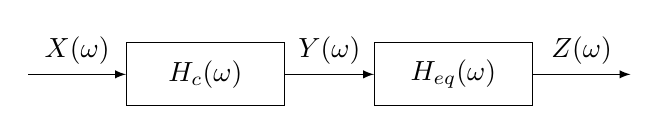
\begin{tikzpicture}[>=latex, scale=0.9]
\node[draw, rectangle, minimum width=2cm, minimum height=0.8cm] (canal) at (0,0) {$H_c(\omega)$};
\node[draw, rectangle, minimum width=2cm, minimum height=0.8cm] (eq) at (3.5,0) {$H_{eq}(\omega)$};
\draw[->] (-2.5,0) -- node[above] {$X(\omega)$} (canal.west);
\draw[->] (canal.east) -- node[above] {$Y(\omega)$} (eq.west);
\draw[->] (eq.east) -- node[above] {$Z(\omega)$} (6,0);
\end{tikzpicture}
\end{center}

\textbf{Função de transferência total:}

\[
Z(\omega) = H_{eq}(\omega) \cdot H_c(\omega) \cdot X(\omega)
\]

\textbf{Condição ideal:}

\[
H_{eq}(\omega) \cdot H_c(\omega) = K e^{-j\omega t_d}
\]

Portanto:
\[
H_{eq}(\omega) = \frac{K e^{-j\omega t_d}}{H_c(\omega)}
\]

\end{frame}

% ============================================

\begin{frame}{Equalização Ideal}

\textbf{Equalizador ideal:}

\[
H_{eq}(\omega) = \frac{1}{H_c(\omega)} = \frac{1}{|H_c(\omega)|} e^{-j\phi_c(\omega)}
\]

\textbf{Efeitos:}

\begin{itemize}
\item \textbf{Equalização de magnitude:} $|H_{eq}(\omega)| = 1/|H_c(\omega)|$
  \begin{itemize}
  \item Frequências atenuadas pelo canal são amplificadas
  \item Frequências amplificadas pelo canal são atenuadas
  \end{itemize}

\item \textbf{Equalização de fase:} $\phi_{eq}(\omega) = -\phi_c(\omega)$
  \begin{itemize}
  \item Cancela a fase não-linear do canal
  \item Restaura relações de fase corretas
  \end{itemize}
\end{itemize}

\vspace{0.3cm}

\textbf{Limitações práticas:}

\begin{itemize}
\item $H_c(\omega)$ deve ser conhecido (estimação de canal)
\item Não pode ser zero em nenhuma frequência (divisão por zero)
\item Amplifica ruído onde $|H_c(\omega)|$ é pequeno
\item Pode ser não-causal se $H_c(\omega)$ não for de fase mínima
\end{itemize}

\end{frame}

% ============================================

\begin{frame}{Tipos de Equalizadores}

\begin{enumerate}
\item \textbf{Equalizador Fixo:}
   \begin{itemize}
   \item Projetado para canal conhecido e estático
   \item Coeficientes fixos
   \item Simples, baixo custo
   \item Exemplo: cabo de comprimento conhecido
   \end{itemize}

\item \textbf{Equalizador Adaptativo:}
   \begin{itemize}
   \item Ajusta coeficientes automaticamente
   \item Rastreia variações do canal
   \item Usa sequência de treinamento ou decisões
   \item Algoritmos: LMS, RLS, CMA
   \item Aplicação: canais móveis, fibra óptica
   \end{itemize}

\item \textbf{Equalizador de Decisão Realimentada (DFE):}
   \begin{itemize}
   \item Usa decisões passadas para cancelar ISI
   \item Não amplifica ruído em frequências com $|H_c| \approx 0$
   \item Mais eficiente em canais com zeros espectrais
   \end{itemize}
\end{enumerate}

\end{frame}

% ============================================

\subsection{Exemplos Práticos}

\begin{frame}{Exemplo 1: Canal Telefônico}

\textbf{Características típicas do canal telefônico (PSTN):}

\begin{itemize}
\item Banda nominal: 300 Hz a 3400 Hz
\item Atenuação: aumenta com frequência (skin effect)
\item Fase: não-linear próximo aos extremos da banda
\item Atraso de grupo: variação de até 2 ms na banda
\end{itemize}

\vspace{0.3cm}

\textbf{Modelo simplificado:}

\[
|H_c(f)| \approx e^{-\alpha f} \quad \text{para} \quad 300 \text{ Hz} < f < 3400 \text{ Hz}
\]

com $\alpha$ dependendo do comprimento do cabo.

\vspace{0.3cm}

\textbf{Equalização:}

Modems de linha discada (V.32, V.34, V.90) usam equalizadores adaptativos complexos para atingir taxas de 28.8-56 kbps nesta banda limitada e distorcida.

\end{frame}

% ============================================

\begin{frame}{Exemplo 2: Canal em Cabo Coaxial}

\textbf{Características de cabo coaxial (TV a cabo, Ethernet):}

\begin{itemize}
\item Atenuação: $\alpha(f) = k_1\sqrt{f} + k_2 f$ (dB/km)
  \begin{itemize}
  \item Termo $\sqrt{f}$: perdas dielétricas
  \item Termo $f$: efeito pelicular (skin effect)
  \end{itemize}
\item Fase: aproximadamente linear
\item Dispersão: mínima em frequências mais baixas
\end{itemize}

\vspace{0.3cm}

\textbf{Exemplo numérico:} RG-59 a 100 MHz e 1 km

Atenuação $\approx 20$ dB $\rightarrow$ $|H_c| \approx 0.1$

\textbf{Equalização:}

Amplificadores em linha com resposta pré-distorcida:

\[
|H_{amp}(f)| \propto \sqrt{f} \quad \text{ou} \quad |H_{amp}(f)| \propto f
\]

Compensa a atenuação crescente do cabo.

\end{frame}

% ============================================

\begin{frame}{Exemplo 3: Canal sem Fio com Multipercurso}

\textbf{Efeito multipercurso:}

Sinal chega ao receptor por múltiplos caminhos com diferentes atrasos e atenuações.

\textbf{Modelo de canal:}

\[
h_c(t) = \sum_{i=1}^{N} a_i \delta(t - \tau_i)
\]

\textbf{Resposta em frequência:}

\[
H_c(\omega) = \sum_{i=1}^{N} a_i e^{-j\omega\tau_i}
\]

\textbf{Características:}

\begin{itemize}
\item \textbf{Desvanecimento seletivo em frequência:} $|H_c(\omega)|$ varia rapidamente
\item Frequências onde há interferência destrutiva: $|H_c(\omega)| \approx 0$ (nulls)
\item Atraso de grupo altamente variável
\item Canal varia com tempo (movimento)
\end{itemize}

\textbf{Equalização:} Adaptativa complexa, OFDM para contornar desvanecimento.

\end{frame}

% ============================================

\begin{frame}{Compromisso: Equalização versus Ruído}

\textbf{Problema fundamental:}

Equalização amplifica sinal \textbf{E} ruído nas frequências atenuadas pelo canal.

\textbf{Análise:}

Canal: $Y(\omega) = H_c(\omega)X(\omega) + N(\omega)$

Após equalização: $Z(\omega) = H_{eq}(\omega)Y(\omega)$

\[
Z(\omega) = H_{eq}(\omega)H_c(\omega)X(\omega) + H_{eq}(\omega)N(\omega)
\]

Se $|H_c(\omega_0)| \approx 0$ (null espectral):

\begin{itemize}
\item Equalizador requer $|H_{eq}(\omega_0)| \to \infty$
\item Ruído nessa frequência é amplificado enormemente
\item SNR deteriora drasticamente
\end{itemize}

\vspace{0.3cm}

\textbf{Solução:} Equalização de mínimo erro quadrático médio (MMSE) que balanceia distorção residual vs. amplificação de ruído.

\end{frame}

% ============================================

\begin{frame}{Resumo da Seção 3.6}

\textbf{Tipos de distorção em canais:}

\begin{itemize}
\item \textbf{Distorção de amplitude:} $|H_c(\omega)|$ variável
\item \textbf{Distorção de fase:} $\phi_c(\omega)$ não-linear
\item Ambas alteram formato do sinal
\end{itemize}

\vspace{0.3cm}

\textbf{Atraso de grupo:} $\tau_g(\omega) = -d\phi_c/d\omega$

Deve ser constante para evitar distorção de fase.

\vspace{0.3cm}

\textbf{Equalização:}

\begin{itemize}
\item Compensa distorção: $H_{eq}(\omega) \approx 1/H_c(\omega)$
\item Pode ser fixa ou adaptativa
\item Compromisso: correção vs. amplificação de ruído
\end{itemize}

\vspace{0.3cm}

\textbf{Aplicações práticas:} Telefonia, TV a cabo, comunicação sem fio.

\end{frame}


% ============================================
% SEÇÃO 3.7: ENERGIA E DENSIDADE ESPECTRAL DE ENERGIA
% ============================================
\section{Energia de Sinal e Densidade Espectral de Energia}
% ============================================
% SEÇÃO 3.7: ENERGIA E DENSIDADE ESPECTRAL DE ENERGIA
% ============================================

\subsection{Energia de Sinais}

\begin{frame}{Classificação de Sinais por Energia e Potência}

Sinais podem ser classificados em duas categorias:

\begin{enumerate}
\item \textbf{Sinais de Energia:}
   \begin{itemize}
   \item Energia finita: $0 < E < \infty$
   \item Potência média: $P = 0$
   \item Exemplos: pulsos, sinais transitórios, sinais causais decrescentes
   \end{itemize}

\item \textbf{Sinais de Potência:}
   \begin{itemize}
   \item Energia infinita: $E = \infty$
   \item Potência média finita: $0 < P < \infty$
   \item Exemplos: sinais periódicos, constantes, aleatórios estacionários
   \end{itemize}
\end{enumerate}

\vspace{0.3cm}

\textbf{Nota:} Alguns sinais (como $t$ ou $e^t$) não se enquadram em nenhuma categoria: energia e potência infinitas.

\textbf{Foco desta seção:} Sinais de energia.

\end{frame}

% ============================================

\begin{frame}{Energia de um Sinal no Domínio do Tempo}

A \textbf{energia} de um sinal $f(t)$ é definida como:

\[
E = \int_{-\infty}^{\infty} |f(t)|^2 dt
\]

\textbf{Interpretação física:}

\begin{itemize}
\item Para sinal de tensão $v(t)$ em resistor de 1 $\Omega$: energia dissipada
\item $|f(t)|^2$ é a potência instantânea
\item Integral acumula energia total ao longo do tempo
\end{itemize}

\vspace{0.3cm}

\textbf{Unidades:}

\begin{itemize}
\item Se $f(t)$ é tensão em volts: energia em joules
\item Se $f(t)$ é normalizado: energia adimensional
\end{itemize}

\vspace{0.3cm}

\textbf{Para sinais complexos:} $|f(t)|^2 = f(t) \cdot f^*(t)$ onde $f^*(t)$ é o conjugado complexo.

\end{frame}

% ============================================

\begin{frame}{Exemplos: Energia de Sinais}

\textbf{Exemplo 1: Pulso retangular}

$f(t) = A\rect(t/\tau)$

\[
E = \int_{-\tau/2}^{\tau/2} A^2 dt = A^2\tau
\]

Energia proporcional à amplitude ao quadrado e à duração.

\vspace{0.3cm}

\textbf{Exemplo 2: Exponencial decrescente}

$f(t) = e^{-at}u(t)$, $a > 0$

\[
E = \int_{0}^{\infty} e^{-2at} dt = \left[-\frac{e^{-2at}}{2a}\right]_0^{\infty} = \frac{1}{2a}
\]

Energia inversamente proporcional à taxa de decaimento.

\vspace{0.3cm}

\textbf{Exemplo 3: Senoide}

$f(t) = A\cos(\omega_0 t)$ (para todo $t$)

\[
E = \int_{-\infty}^{\infty} A^2\cos^2(\omega_0 t) dt = \infty
\]

Sinal periódico tem energia infinita (é sinal de potência).

\end{frame}

% ============================================

\subsection{Teorema de Parseval}

\begin{frame}{Energia no Domínio da Frequência}

\textbf{Teorema de Parseval} relaciona energia nos domínios do tempo e frequência.

\begin{block}{Teorema de Parseval}
Se $f(t) \xleftrightarrow{\ft} F(\omega)$, então:
\[
E = \int_{-\infty}^{\infty} |f(t)|^2 dt = \frac{1}{2\pi} \int_{-\infty}^{\infty} |F(\omega)|^2 d\omega
\]
\end{block}

\textbf{Significado:}

\begin{itemize}
\item A energia total é a mesma calculada no tempo ou na frequência
\item A energia é conservada entre os domínios
\item $|F(\omega)|^2/(2\pi)$ representa densidade de energia por unidade de frequência
\end{itemize}

\vspace{0.3cm}

\textbf{Analogia:} Como a energia total de um sistema físico permanece constante em diferentes sistemas de coordenadas.

\end{frame}

% ============================================

\begin{frame}{Demonstração do Teorema de Parseval (revisão)}

Começamos com a definição de energia:

\[
E = \int_{-\infty}^{\infty} |f(t)|^2 dt = \int_{-\infty}^{\infty} f(t) f^*(t) dt
\]

Substituindo a transformada inversa para $f^*(t)$:

\[
f^*(t) = \left[\frac{1}{2\pi} \int_{-\infty}^{\infty} F(\omega) e^{j\omega t} d\omega\right]^* = \frac{1}{2\pi} \int_{-\infty}^{\infty} F^*(\omega) e^{-j\omega t} d\omega
\]

Portanto:

\[
E = \int_{-\infty}^{\infty} f(t) \left[\frac{1}{2\pi} \int_{-\infty}^{\infty} F^*(\omega) e^{-j\omega t} d\omega\right] dt
\]

Trocando a ordem de integração:

\[
E = \frac{1}{2\pi} \int_{-\infty}^{\infty} F^*(\omega) \left[\int_{-\infty}^{\infty} f(t) e^{-j\omega t} dt\right] d\omega
\]

\end{frame}

% ============================================

\begin{frame}{Demonstração do Teorema de Parseval (conclusão)}

A integral interna é justamente $F(\omega)$:

\[
E = \frac{1}{2\pi} \int_{-\infty}^{\infty} F^*(\omega) F(\omega) d\omega
\]

\[
= \frac{1}{2\pi} \int_{-\infty}^{\infty} |F(\omega)|^2 d\omega
\]

Portanto:

\[
\boxed{\int_{-\infty}^{\infty} |f(t)|^2 dt = \frac{1}{2\pi} \int_{-\infty}^{\infty} |F(\omega)|^2 d\omega}
\]

\textbf{Conclusão:} A energia pode ser calculada em qualquer domínio, com resultado idêntico.

\textbf{Importância prática:} Às vezes é mais fácil calcular energia na frequência que no tempo.

\end{frame}

% ============================================

\subsection{Densidade Espectral de Energia}

\begin{frame}{Definição de Densidade Espectral de Energia}

A \textbf{Densidade Espectral de Energia (DEE)} ou \textit{Energy Spectral Density (ESD)} é definida como:

\begin{block}{Densidade Espectral de Energia}
\[
\Psi(\omega) = |F(\omega)|^2
\]
\end{block}

\textbf{Unidades:} Energia por Hz (ou por rad/s, dependendo se usa $f$ ou $\omega$).

\textbf{Interpretação:}

\begin{itemize}
\item $\Psi(\omega)$ indica quanto de energia está concentrado em cada frequência
\item Áreas sob $\Psi(\omega)$ representam energia em bandas de frequência
\item Pelo Teorema de Parseval:
\[
E = \frac{1}{2\pi} \int_{-\infty}^{\infty} \Psi(\omega) d\omega
\]
\end{itemize}

\textbf{Propriedade:} Para sinais reais, $\Psi(\omega)$ é par: $\Psi(-\omega) = \Psi(\omega)$

\end{frame}

% ============================================

\begin{frame}{Exemplo: DEE de Pulso Retangular}

\textbf{Sinal:} $f(t) = A\rect(t/\tau)$

Já sabemos que:
\[
F(\omega) = A\tau \sinc\left(\frac{\omega\tau}{2\pi}\right)
\]

\textbf{Densidade espectral de energia:}

\[
\Psi(\omega) = |F(\omega)|^2 = A^2\tau^2 \sinc^2\left(\frac{\omega\tau}{2\pi}\right)
\]

\textbf{Características:}

\begin{itemize}
\item Máximo em $\omega = 0$: $\Psi(0) = A^2\tau^2$
\item Zeros em $\omega = \pm 2\pi n/\tau$ para $n = 1, 2, 3, ...$
\item Maior parte da energia no lóbulo principal: $|\omega| < 2\pi/\tau$
\item Decai como $1/\omega^2$ para grandes $\omega$
\end{itemize}

\textbf{Verificação do Teorema de Parseval:} A integral de $\Psi(\omega)/(2\pi)$ deve dar $A^2\tau$ (energia no tempo).

\end{frame}

% ============================================

\begin{frame}{Exemplo: DEE de Exponencial Decrescente}

\textbf{Sinal:} $f(t) = e^{-at}u(t)$, $a > 0$

Transformada:
\[
F(\omega) = \frac{1}{a + j\omega}
\]

\textbf{Densidade espectral de energia:}

\[
\Psi(\omega) = |F(\omega)|^2 = \frac{1}{|a + j\omega|^2} = \frac{1}{a^2 + \omega^2}
\]

\textbf{Características:}

\begin{itemize}
\item Forma Lorentziana
\item Máximo em $\omega = 0$: $\Psi(0) = 1/a^2$
\item Em $\omega = \pm a$: $\Psi(a) = 1/(2a^2)$ (metade do máximo)
\item Decai como $1/\omega^2$ para $\omega \to \infty$
\end{itemize}

\textbf{Energia total:}

\[
E = \frac{1}{2\pi} \int_{-\infty}^{\infty} \frac{1}{a^2 + \omega^2} d\omega = \frac{1}{2\pi} \cdot \frac{2\pi}{2a} = \frac{1}{2a}
\]

Confirma cálculo no tempo!

\end{frame}

% ============================================

\subsection{Largura de Banda de Energia}

\begin{frame}{Conceito de Largura de Banda}

A \textbf{largura de banda} de um sinal quantifica a faixa de frequências que contém sua energia significativa.

\textbf{Definições comuns:}

\begin{enumerate}
\item \textbf{Largura de banda absoluta:}
   
   Menor intervalo $[-W, W]$ onde $F(\omega) \neq 0$
   
   (pode ser infinita)

\item \textbf{Largura de banda de 3 dB:}
   
   Faixa onde $\Psi(\omega) \geq \Psi_{\max}/2$

\item \textbf{Largura de banda de ruído:}
   
   Largura de um retângulo equivalente de mesma área e altura máxima:
   \[
   B_n = \frac{1}{\Psi(0)} \int_{-\infty}^{\infty} \Psi(\omega) d\omega = \frac{2\pi E}{\Psi(0)}
   \]

\item \textbf{Largura de banda de X\%:}
   
   Menor faixa $[-W_x, W_x]$ contendo X\% da energia total
\end{enumerate}

\end{frame}

% ============================================

\begin{frame}{Cálculo de Largura de Banda de X\%}

\textbf{Definição:} Encontrar $W_x$ tal que:

\[
\frac{1}{2\pi} \int_{-W_x}^{W_x} \Psi(\omega) d\omega = \alpha E
\]

onde $\alpha$ é a fração desejada (ex: 0.90 para 90\%, 0.99 para 99\%).

\vspace{0.3cm}

\textbf{Exemplo: Pulso retangular}

Para $f(t) = \rect(t/\tau)$ com $\Psi(\omega) = \tau^2 \sinc^2(\omega\tau/2\pi)$:

\begin{itemize}
\item Lóbulo principal ($|\omega| < 2\pi/\tau$) contém $\approx 90\%$ da energia
\item $W_{90\%} \approx 2\pi/\tau$ ou $B_{90\%} \approx 1/\tau$ em Hz
\end{itemize}

\textbf{Princípio geral:}

\[
\text{Duração no tempo} \times \text{Largura de banda} \approx \text{constante}
\]

Pulso mais curto $\rightarrow$ espectro mais largo.

\end{frame}

% ============================================

\subsection{Relação de Incerteza}

\begin{frame}{Desigualdade de Heisenberg-Gabor}

\textbf{Duração efetiva} de um sinal:

\[
\Delta t = \sqrt{\frac{\int_{-\infty}^{\infty} t^2 |f(t)|^2 dt}{\int_{-\infty}^{\infty} |f(t)|^2 dt}}
\]

\textbf{Largura de banda efetiva:}

\[
\Delta \omega = \sqrt{\frac{\int_{-\infty}^{\infty} \omega^2 |F(\omega)|^2 d\omega}{\int_{-\infty}^{\infty} |F(\omega)|^2 d\omega}}
\]

\begin{block}{Desigualdade de Heisenberg-Gabor}
\[
\Delta t \cdot \Delta \omega \geq \frac{1}{2}
\]
\end{block}

\textbf{Significado:}

\begin{itemize}
\item Produto tempo-frequência tem limite inferior
\item Não podemos ter sinal arbitrariamente concentrado em ambos os domínios
\item Compromisso fundamental: localização no tempo $\leftrightarrow$ localização em frequência
\end{itemize}

\end{frame}

% ============================================

\begin{frame}{Sinal Ótimo: Gaussiana}

O \textbf{pulso Gaussiano} atinge a igualdade na desigualdade:

\[
f(t) = e^{-\alpha t^2} \quad \xleftrightarrow{\ft} \quad F(\omega) = \sqrt{\frac{\pi}{\alpha}} e^{-\omega^2/(4\alpha)}
\]

Para este sinal:

\[
\Delta t \cdot \Delta \omega = \frac{1}{2}
\]

\textbf{Propriedades da Gaussiana:}

\begin{itemize}
\item Gaussiana no tempo $\leftrightarrow$ Gaussiana na frequência
\item Melhor localização simultânea tempo-frequência
\item Mínima incerteza
\item Usada em comunicações ópticas e rádio
\end{itemize}

\vspace{0.3cm}

\textbf{Todos os outros sinais:} $\Delta t \cdot \Delta \omega > 1/2$

\end{frame}

% ============================================

\subsection{Energia na Saída de Sistemas LTI}

\begin{frame}{Energia através de Sistema LTI}

\textbf{Sistema:} Entrada $x(t)$ com transformada $X(\omega)$, saída $y(t)$.

\textbf{Relação:} $Y(\omega) = H(\omega) X(\omega)$

\textbf{Energia da entrada:}

\[
E_x = \frac{1}{2\pi} \int_{-\infty}^{\infty} |X(\omega)|^2 d\omega
\]

\textbf{Energia da saída:}

\[
E_y = \frac{1}{2\pi} \int_{-\infty}^{\infty} |Y(\omega)|^2 d\omega = \frac{1}{2\pi} \int_{-\infty}^{\infty} |H(\omega)|^2 |X(\omega)|^2 d\omega
\]

\begin{block}{Relação Entrada-Saída}
\[
\Psi_y(\omega) = |H(\omega)|^2 \Psi_x(\omega)
\]
\end{block}

\textbf{Interpretação:} A DEE da saída é a DEE da entrada multiplicada pelo quadrado da magnitude da resposta em frequência.

\end{frame}

% ============================================

\begin{frame}{Exemplo: Pulso através de Filtro RC}

\textbf{Entrada:} Pulso $x(t) = \delta(t)$ (impulso unitário)

$X(\omega) = 1$, $\Psi_x(\omega) = 1$

\textbf{Sistema:} Filtro RC passa-baixas

\[
H(\omega) = \frac{1}{1 + j\omega RC}
\]

\textbf{DEE da saída:}

\[
\Psi_y(\omega) = |H(\omega)|^2 = \frac{1}{1 + (\omega RC)^2}
\]

\textbf{Energia da saída:}

\[
E_y = \frac{1}{2\pi} \int_{-\infty}^{\infty} \frac{1}{1 + (\omega RC)^2} d\omega
\]

Com $\omega_c = 1/(RC)$:

\[
E_y = \frac{1}{2\pi} \cdot \frac{2\pi}{\omega_c \cdot 2} = \frac{1}{2\omega_c} = \frac{RC}{2}
\]

\end{frame}

% ============================================

\begin{frame}{Energia em Banda Limitada}

\textbf{Problema:} Qual fração da energia passa por um filtro passa-baixas ideal?

\textbf{Filtro:} $H(\omega) = \rect(\omega/2W)$ com largura de banda $W$

\textbf{Energia transmitida:}

\[
E_{pass} = \frac{1}{2\pi} \int_{-W}^{W} \Psi_x(\omega) d\omega
\]

\textbf{Fração da energia:}

\[
\eta = \frac{E_{pass}}{E_{total}} = \frac{\int_{-W}^{W} \Psi_x(\omega) d\omega}{\int_{-\infty}^{\infty} \Psi_x(\omega) d\omega}
\]

\vspace{0.3cm}

\textbf{Exemplo: Exponencial} $e^{-a|t|}$ com $\Psi(\omega) = 4a^2/(a^2+\omega^2)^2$

Para $W = 3a$: $\eta \approx 0.95$ (95\% da energia dentro de $[-3a, 3a]$)

\textbf{Aplicação:} Projeto de sistemas com banda limitada.

\end{frame}

% ============================================

\subsection{Autocorrelação e DEE}

\begin{frame}{Função de Autocorrelação}

A \textbf{função de autocorrelação} de um sinal de energia $f(t)$ é:

\[
R(\tau) = \int_{-\infty}^{\infty} f(t) f^*(t - \tau) dt
\]

\textbf{Propriedades:}

\begin{itemize}
\item $R(0) = E$ (energia total)
\item $R(\tau) = R^*(-\tau)$ (simetria Hermitiana)
\item Para sinais reais: $R(\tau) = R(-\tau)$ (par)
\item $|R(\tau)| \leq R(0) = E$
\end{itemize}

\vspace{0.3cm}

\textbf{Interpretação:} Mede similaridade do sinal com versão deslocada de si mesmo.

\begin{block}{Teorema de Wiener-Khinchin (Energia)}
\[
R(\tau) \xleftrightarrow{\ft} \Psi(\omega) = |F(\omega)|^2
\]
\end{block}

A autocorrelação e a DEE são pares de Fourier!

\end{frame}

% ============================================

\begin{frame}{Resumo da Seção 3.7}

\textbf{Conceitos fundamentais:}

\begin{itemize}
\item \textbf{Energia no tempo:} $E = \int |f(t)|^2 dt$
\item \textbf{Energia na frequência:} $E = \frac{1}{2\pi}\int |F(\omega)|^2 d\omega$
\item \textbf{Teorema de Parseval:} Energia conservada entre domínios
\end{itemize}

\vspace{0.3cm}

\textbf{Densidade Espectral de Energia:}

\begin{itemize}
\item $\Psi(\omega) = |F(\omega)|^2$
\item Indica distribuição de energia em frequência
\item Em sistemas LTI: $\Psi_y(\omega) = |H(\omega)|^2 \Psi_x(\omega)$
\end{itemize}

\vspace{0.3cm}

\textbf{Princípios importantes:}

\begin{itemize}
\item Relação de incerteza: $\Delta t \cdot \Delta \omega \geq 1/2$
\item Gaussiana é ótima (atinge igualdade)
\item Largura de banda relacionada com duração temporal
\end{itemize}

\textbf{Próximo:} Sinais de potência e densidade espectral de potência.

\end{frame}


% ============================================
% SEÇÃO 3.8: POTÊNCIA E DENSIDADE ESPECTRAL DE POTÊNCIA
% ============================================
\section{Potência de Sinal e Densidade Espectral de Potência}
% ============================================
% SEÇÃO 3.8: POTÊNCIA E DENSIDADE ESPECTRAL DE POTÊNCIA
% ============================================

\subsection{Sinais de Potência}

\begin{frame}{Potência Média de um Sinal}

Para sinais que não têm energia finita (sinais de potência), define-se a \textbf{potência média}:

\[
P = \lim_{T \to \infty} \frac{1}{T} \int_{-T/2}^{T/2} |f(t)|^2 dt
\]

\textbf{Exemplos de sinais de potência:}

\begin{itemize}
\item Sinais periódicos: $\cos(\omega_0 t)$, ondas quadradas
\item Constantes: $f(t) = A$
\item Sinais aleatórios estacionários: ruído branco, processos ergódicos
\end{itemize}

\vspace{0.3cm}

\textbf{Diferença fundamental:}

\begin{center}
\begin{tabular}{|l|c|c|}
\hline
& \textbf{Energia} & \textbf{Potência} \\
\hline
Sinais de energia & Finita & Zero \\
Sinais de potência & Infinita & Finita \\
\hline
\end{tabular}
\end{center}

\textbf{Nota:} $P$ tem unidades de watts (ou normalizadas).

\end{frame}

% ============================================

\begin{frame}{Exemplos: Potência de Sinais}

\textbf{Exemplo 1: Senoide}

$f(t) = A\cos(\omega_0 t)$

\[
P = \lim_{T \to \infty} \frac{1}{T} \int_{-T/2}^{T/2} A^2\cos^2(\omega_0 t) dt
\]

Usando $\cos^2(\theta) = (1 + \cos(2\theta))/2$ e integrando sobre período inteiro:

\[
P = A^2 \cdot \frac{1}{2} = \frac{A^2}{2}
\]

\vspace{0.3cm}

\textbf{Exemplo 2: Constante}

$f(t) = A$

\[
P = \lim_{T \to \infty} \frac{1}{T} \int_{-T/2}^{T/2} A^2 dt = A^2
\]

\vspace{0.3cm}

\textbf{Exemplo 3: Onda quadrada periódica}

Amplitude $\pm A$, período $T_0$: $P = A^2$

\end{frame}

% ============================================

\subsection{Densidade Espectral de Potência}

\begin{frame}{Necessidade da PSD}

\textbf{Problema:} Para sinais de potência, a transformada de Fourier padrão não existe!

Para $f(t) = A\cos(\omega_0 t)$:

\[
\int_{-\infty}^{\infty} |A\cos(\omega_0 t)| dt = \infty
\]

Não satisfaz condição de Dirichlet.

\vspace{0.3cm}

\textbf{Solução:} Usar funções generalizadas (distribuições) ou definir potência no domínio da frequência através da \textbf{Densidade Espectral de Potência (PSD)}.

\textbf{PSD} $S(\omega)$ indica como a potência está distribuída em frequência.

\vspace{0.3cm}

\textbf{Relação fundamental:}

\[
P = \frac{1}{2\pi} \int_{-\infty}^{\infty} S(\omega) d\omega
\]

\end{frame}

% ============================================

\begin{frame}{Definição da PSD}

Para um sinal de potência $f(t)$, define-se:

\textbf{Sinal truncado:}

\[
f_T(t) = \begin{cases}
f(t) & |t| \leq T/2 \\
0 & |t| > T/2
\end{cases}
\]

$f_T(t)$ tem energia finita, logo possui transformada $F_T(\omega)$.

\begin{block}{Densidade Espectral de Potência}
\[
S(\omega) = \lim_{T \to \infty} \frac{1}{T} |F_T(\omega)|^2 = \lim_{T \to \infty} \frac{|F_T(\omega)|^2}{T}
\]
\end{block}

\textbf{Interpretação:}

\begin{itemize}
\item DEE normalizada pelo tempo de observação
\item $S(\omega)$ tem unidades de potência por Hz
\item Indica distribuição de potência no espectro
\end{itemize}

\end{frame}

% ============================================

\begin{frame}{PSD de Sinais Periódicos}

Para sinal periódico com série de Fourier:

\[
f(t) = \sum_{n=-\infty}^{\infty} c_n e^{jn\omega_0 t}
\]

A PSD é:

\begin{block}{PSD de Sinal Periódico}
\[
S(\omega) = 2\pi \sum_{n=-\infty}^{\infty} |c_n|^2 \delta(\omega - n\omega_0)
\]
\end{block}

\textbf{Características:}

\begin{itemize}
\item Espectro discreto (impulsos nas harmônicas)
\item Impulsos localizados em $\omega = n\omega_0$
\item Área de cada impulso: $2\pi|c_n|^2$ (potência naquela harmônica)
\item Potência total: $P = \sum_{n=-\infty}^{\infty} |c_n|^2$
\end{itemize}

\textbf{Significado físico:} Sinal periódico tem potência concentrada em frequências discretas.

\end{frame}

% ============================================

\begin{frame}{Exemplo: PSD de Senoide}

\textbf{Sinal:} $f(t) = A\cos(\omega_0 t)$

Escrevendo em forma exponencial:

\[
f(t) = \frac{A}{2} e^{j\omega_0 t} + \frac{A}{2} e^{-j\omega_0 t}
\]

Coeficientes: $c_1 = c_{-1} = A/2$, $c_n = 0$ para $n \neq \pm 1$

\textbf{PSD:}

\[
S(\omega) = 2\pi \left[\left|\frac{A}{2}\right|^2 \delta(\omega - \omega_0) + \left|\frac{A}{2}\right|^2 \delta(\omega + \omega_0)\right]
\]

\[
= \frac{\pi A^2}{2} [\delta(\omega - \omega_0) + \delta(\omega + \omega_0)]
\]

\textbf{Potência total:}

\[
P = \frac{1}{2\pi} \cdot \frac{\pi A^2}{2} \cdot 2 = \frac{A^2}{2}
\]

Confirma cálculo no tempo!

\end{frame}

% ============================================

\subsection{Autocorrelação e Teorema de Wiener-Khinchin}

\begin{frame}{Função de Autocorrelação para Sinais de Potência}

A \textbf{função de autocorrelação} para um sinal de potência é:

\[
R(\tau) = \lim_{T \to \infty} \frac{1}{T} \int_{-T/2}^{T/2} f(t) f^*(t - \tau) dt
\]

\textbf{Propriedades:}

\begin{itemize}
\item $R(0) = P$ (potência média)
\item $R(\tau) = R^*(-\tau)$ (simetria Hermitiana)
\item Para sinais reais: $R(\tau) = R(-\tau)$ (par)
\item $|R(\tau)| \leq R(0) = P$
\end{itemize}

\vspace{0.3cm}

\textbf{Interpretação física:}

\begin{itemize}
\item Mede correlação temporal do sinal
\item $R(\tau)$ grande $\rightarrow$ valores em $t$ e $t+\tau$ correlacionados
\item $R(\tau)$ pequeno $\rightarrow$ valores descorrelacionados
\end{itemize}

\end{frame}

% ============================================

\begin{frame}{Teorema de Wiener-Khinchin}

\begin{block}{Teorema de Wiener-Khinchin}
A PSD e a função de autocorrelação formam um par de transformadas de Fourier:
\[
R(\tau) \xleftrightarrow{\ft} S(\omega)
\]

Ou seja:
\[
S(\omega) = \int_{-\infty}^{\infty} R(\tau) e^{-j\omega\tau} d\tau
\]
\[
R(\tau) = \frac{1}{2\pi} \int_{-\infty}^{\infty} S(\omega) e^{j\omega\tau} d\omega
\]
\end{block}

\textbf{Importância:}

\begin{itemize}
\item Relaciona propriedades temporais (correlação) com espectrais (potência)
\item PSD pode ser calculada via autocorrelação
\item Fundamental em processamento de sinais aleatórios
\item Base para análise espectral não-paramétrica
\end{itemize}

\end{frame}

% ============================================

\begin{frame}{Demonstração do Teorema (esboço)}

Começando com a definição de PSD:

\[
S(\omega) = \lim_{T \to \infty} \frac{|F_T(\omega)|^2}{T}
\]

Expandindo $|F_T(\omega)|^2 = F_T(\omega) F_T^*(\omega)$:

\[
|F_T(\omega)|^2 = \int_{-T/2}^{T/2} f_T(t) e^{-j\omega t} dt \int_{-T/2}^{T/2} f_T^*(t') e^{j\omega t'} dt'
\]

Combinando as integrais e mudando variável $\tau = t - t'$:

\[
|F_T(\omega)|^2 = \int \int f_T(t) f_T^*(t') e^{-j\omega(t-t')} dt' dt
\]

Após manipulação e tomando limite $T \to \infty$:

\[
S(\omega) = \int_{-\infty}^{\infty} \left[\lim_{T \to \infty} \frac{1}{T} \int f(t) f^*(t-\tau) dt\right] e^{-j\omega\tau} d\tau
\]

\[
= \int_{-\infty}^{\infty} R(\tau) e^{-j\omega\tau} d\tau
\]

\end{frame}

% ============================================

\begin{frame}{Exemplo: Autocorrelação de Senoide}

\textbf{Sinal:} $f(t) = A\cos(\omega_0 t)$

\textbf{Autocorrelação:}

\[
R(\tau) = \lim_{T \to \infty} \frac{1}{T} \int_{-T/2}^{T/2} A\cos(\omega_0 t) \cdot A\cos(\omega_0(t-\tau)) dt
\]

Usando identidade $\cos(a)\cos(b) = \frac{1}{2}[\cos(a-b) + \cos(a+b)]$:

\[
R(\tau) = \lim_{T \to \infty} \frac{A^2}{2T} \int_{-T/2}^{T/2} [\cos(\omega_0 \tau) + \cos(2\omega_0 t - \omega_0\tau)] dt
\]

O segundo termo integra a zero sobre período completo:

\[
R(\tau) = \frac{A^2}{2} \cos(\omega_0 \tau)
\]

\textbf{Transformada:}

\[
S(\omega) = \frac{A^2}{2} \FT{\cos(\omega_0 \tau)} = \frac{\pi A^2}{2}[\delta(\omega - \omega_0) + \delta(\omega + \omega_0)]
\]

Confirma resultado anterior!

\end{frame}

% ============================================

\subsection{PSD na Saída de Sistemas LTI}

\begin{frame}{Transformação de PSD por Sistema LTI}

\textbf{Sistema:} Entrada $x(t)$ com PSD $S_x(\omega)$, saída $y(t)$ com PSD $S_y(\omega)$.

\textbf{Relação na frequência:} $Y(\omega) = H(\omega) X(\omega)$

\textbf{Derivação:}

Para sinal truncado: $Y_T(\omega) = H(\omega) X_T(\omega)$

\[
|Y_T(\omega)|^2 = |H(\omega)|^2 |X_T(\omega)|^2
\]

Tomando limite:

\[
S_y(\omega) = \lim_{T \to \infty} \frac{|Y_T(\omega)|^2}{T} = |H(\omega)|^2 \lim_{T \to \infty} \frac{|X_T(\omega)|^2}{T}
\]

\begin{block}{Relação Entrada-Saída para PSD}
\[
\boxed{S_y(\omega) = |H(\omega)|^2 S_x(\omega)}
\]
\end{block}

\textbf{Idêntico à relação para DEE!}

\end{frame}

% ============================================

\begin{frame}{Potência na Saída de Sistema LTI}

A potência na saída é:

\[
P_y = \frac{1}{2\pi} \int_{-\infty}^{\infty} S_y(\omega) d\omega
\]

Substituindo $S_y(\omega) = |H(\omega)|^2 S_x(\omega)$:

\[
P_y = \frac{1}{2\pi} \int_{-\infty}^{\infty} |H(\omega)|^2 S_x(\omega) d\omega
\]

\textbf{Interpretação:}

\begin{itemize}
\item Cada componente espectral da entrada é filtrada por $|H(\omega)|^2$
\item Frequências amplificadas pelo sistema contribuem mais à potência de saída
\item Frequências atenuadas contribuem menos
\end{itemize}

\vspace{0.3cm}

\textbf{Aplicação importante:} Análise de ruído em sistemas de comunicação.

\end{frame}

% ============================================

\subsection{Ruído Branco}

\begin{frame}{Ruído Branco}

\textbf{Ruído branco ideal:} Processo aleatório com PSD constante para todas as frequências.

\begin{block}{PSD de Ruído Branco}
\[
S_n(\omega) = \frac{N_0}{2} \quad \text{para todo} \quad \omega
\]
\end{block}

onde $N_0$ é a densidade espectral de potência bilateral.

\vspace{0.3cm}

\textbf{Características:}

\begin{itemize}
\item Potência infinita: $P = \int_{-\infty}^{\infty} (N_0/2)/(2\pi) d\omega = \infty$
\item Todas as frequências igualmente representadas
\item Analogia: Luz branca contém todas as cores
\item Modelo idealizado (fisicamente irrealizável)
\end{itemize}

\textbf{Autocorrelação:}

\[
R_n(\tau) = \frac{N_0}{2} \delta(\tau)
\]

Amostras em tempos diferentes são completamente descorrelacionadas!

\end{frame}

% ============================================

\begin{frame}{Ruído Branco Filtrado}

\textbf{Situação prática:} Ruído branco passa por filtro (canal, receptor).

\textbf{Entrada:} Ruído branco $n(t)$ com $S_n(\omega) = N_0/2$

\textbf{Saída:} $y(t) = n(t) \conv h(t)$

\textbf{PSD da saída:}

\[
S_y(\omega) = |H(\omega)|^2 \cdot \frac{N_0}{2}
\]

\textbf{Potência do ruído na saída:}

\[
P_y = \frac{1}{2\pi} \int_{-\infty}^{\infty} |H(\omega)|^2 \frac{N_0}{2} d\omega = \frac{N_0}{4\pi} \int_{-\infty}^{\infty} |H(\omega)|^2 d\omega
\]

Pela relação de Parseval:

\[
P_y = \frac{N_0}{2} \int_{-\infty}^{\infty} |h(t)|^2 dt
\]

\textbf{Ruído filtrado já não é branco!} PSD tem forma de $|H(\omega)|^2$.

\end{frame}

% ============================================

\begin{frame}{Exemplo: Ruído Branco em Filtro RC}

\textbf{Filtro:} RC passa-baixas com $H(\omega) = 1/(1 + j\omega RC)$

\textbf{Entrada:} Ruído branco $S_n(\omega) = N_0/2$

\textbf{PSD na saída:}

\[
S_y(\omega) = \frac{N_0/2}{1 + (\omega RC)^2}
\]

\textbf{Potência do ruído na saída:}

\[
P_y = \frac{1}{2\pi} \int_{-\infty}^{\infty} \frac{N_0/2}{1 + (\omega RC)^2} d\omega
\]

Com $\omega_c = 1/(RC)$:

\[
P_y = \frac{N_0}{4\pi} \cdot \frac{2\pi}{\omega_c} = \frac{N_0}{4\omega_c} = \frac{N_0}{4} \cdot RC = \frac{N_0 \cdot BW}{2}
\]

onde $BW = 1/(4RC)$ é a largura de banda de ruído do filtro.

\textbf{Conclusão:} Potência de ruído proporcional à largura de banda!

\end{frame}

% ============================================

\subsection{Relação Sinal-Ruído (SNR)}

\begin{frame}{Relação Sinal-Ruído}

A \textbf{Relação Sinal-Ruído (SNR)} quantifica qualidade do sinal:

\[
\text{SNR} = \frac{P_{\text{sinal}}}{P_{\text{ruído}}}
\]

Em decibéis:

\[
\text{SNR}_{dB} = 10\log_{10}\left(\frac{P_{\text{sinal}}}{P_{\text{ruído}}}\right)
\]

\vspace{0.3cm}

\textbf{Importância:}

\begin{itemize}
\item Medida fundamental de qualidade em comunicações
\item Determina taxa de erro e capacidade do canal
\item SNR alta: comunicação confiável
\item SNR baixa: erros frequentes, degradação
\end{itemize}

\vspace{0.3cm}

\textbf{Valores típicos:}

\begin{itemize}
\item Telefonia analógica: SNR $>$ 30 dB
\item Comunicação digital: SNR $>$ 10-15 dB (depende da modulação)
\item Rádio FM: SNR $>$ 40 dB para boa qualidade
\end{itemize}

\end{frame}

% ============================================

\begin{frame}{SNR em Sistemas de Banda Limitada}

\textbf{Sistema:} Sinal $s(t)$ com potência $P_s$ + ruído branco $n(t)$ com PSD $N_0/2$.

\textbf{Após filtro passa-baixas ideal de largura $W$:}

Potência do sinal: $P_s$ (assumindo sinal banda-limitada em $W$)

Potência do ruído:

\[
P_n = \frac{1}{2\pi} \int_{-W}^{W} \frac{N_0}{2} d\omega = \frac{N_0 \cdot 2W}{4\pi} = \frac{N_0 W}{2\pi}
\]

Em Hz ($f = \omega/2\pi$):

\[
P_n = N_0 B
\]

onde $B = W/(2\pi)$ é a largura de banda em Hz.

\textbf{SNR:}

\[
\text{SNR} = \frac{P_s}{N_0 B}
\]

\textbf{Compromisso:} Aumentar banda $B$ aumenta capacidade mas também aumenta ruído!

\end{frame}

% ============================================

\subsection{Exemplo Integrado}

\begin{frame}{Exemplo: Comunicação em Canal Ruidoso}

\textbf{Sistema:}

\begin{itemize}
\item Sinal transmitido: $s(t) = A\cos(\omega_c t)$, potência $P_s = A^2/2$
\item Canal: Atenuação $\alpha$, ruído branco aditivo $N_0/2$
\item Filtro receptor: Passa-faixas centrado em $\omega_c$, largura $2B$
\end{itemize}

\textbf{Sinal recebido (antes do filtro):}

\[
r(t) = \alpha s(t) + n(t)
\]

\textbf{Após filtro:}

Potência do sinal: $P_{s,out} = \alpha^2 P_s = \alpha^2 A^2/2$

Potência do ruído: $P_{n,out} = N_0 B$ (banda bilateral $2B$, mas simetria)

\textbf{SNR na saída:}

\[
\text{SNR}_{out} = \frac{\alpha^2 A^2/2}{N_0 B} = \frac{\alpha^2 A^2}{2N_0 B}
\]

\end{frame}

% ============================================

\begin{frame}{Resumo da Seção 3.8}

\textbf{Conceitos de potência:}

\begin{itemize}
\item \textbf{Potência média:} $P = \lim_{T\to\infty} \frac{1}{T}\int |f(t)|^2 dt$
\item Para sinais periódicos: $P = \sum |c_n|^2$
\end{itemize}

\vspace{0.3cm}

\textbf{Densidade Espectral de Potência (PSD):}

\begin{itemize}
\item $S(\omega)$: distribuição de potência em frequência
\item $P = \frac{1}{2\pi}\int S(\omega) d\omega$
\item Sinais periódicos: espectro discreto (impulsos)
\end{itemize}

\vspace{0.3cm}

\textbf{Teorema de Wiener-Khinchin:} $R(\tau) \xleftrightarrow{\ft} S(\omega)$

\vspace{0.3cm}

\textbf{Sistemas LTI:} $S_y(\omega) = |H(\omega)|^2 S_x(\omega)$

\vspace{0.3cm}

\textbf{Ruído branco:}

\begin{itemize}
\item PSD constante: $S_n = N_0/2$
\item Após filtragem: potência $\propto$ largura de banda
\item SNR = $P_s/(N_0 B)$
\end{itemize}

\end{frame}


% ============================================
% SEÇÃO 3.9: COMPUTAÇÃO NUMÉRICA DA TRANSFORMADA DE FOURIER
% ============================================
\section{Computação Numérica: DFT e FFT}
% ============================================
% SEÇÃO 3.9: COMPUTAÇÃO NUMÉRICA DA TRANSFORMADA DE FOURIER
% ============================================

\subsection{Motivação}

\begin{frame}{Por que Transformada Discreta?}

\textbf{Transformada de Fourier contínua:}

\[
F(\omega) = \int_{-\infty}^{\infty} f(t) e^{-j\omega t} dt
\]

\textbf{Problemas para implementação computacional:}

\begin{enumerate}
\item \textbf{Integral infinita:} Computadores não processam intervalos infinitos
\item \textbf{Tempo contínuo:} Necessário amostrar o sinal discretamente
\item \textbf{Frequência contínua:} Impossível calcular para todo $\omega$
\end{enumerate}

\vspace{0.3cm}

\textbf{Solução:} \textbf{Transformada Discreta de Fourier (DFT)}

\begin{itemize}
\item Opera em sequências finitas de amostras
\item Produz espectro em frequências discretas
\item Computável em tempo finito
\item Base para análise espectral prática
\end{itemize}

\end{frame}

% ============================================

\subsection{Amostragem de Sinais}

\begin{frame}{Teorema da Amostragem (Nyquist-Shannon)}

\textbf{Problema:} Converter sinal contínuo $f(t)$ em amostras discretas $f[n]$.

\begin{block}{Teorema de Nyquist-Shannon}
Um sinal de banda limitada $f(t)$ com frequência máxima $f_{max}$ pode ser perfeitamente reconstruído a partir de suas amostras se a taxa de amostragem $f_s$ satisfizer:
\[
f_s \geq 2f_{max}
\]
\end{block}

\textbf{Definições:}

\begin{itemize}
\item \textbf{Taxa de Nyquist:} $f_N = 2f_{max}$ (taxa mínima)
\item \textbf{Período de amostragem:} $T_s = 1/f_s$
\item \textbf{Amostras:} $f[n] = f(nT_s)$ para $n = 0, 1, 2, ..., N-1$
\end{itemize}

\vspace{0.3cm}

\textbf{Consequência:} Se $f_s < 2f_{max}$, ocorre \textbf{aliasing} (distorção espectral).

\end{frame}

% ============================================

\begin{frame}{Aliasing}

\textbf{Aliasing} ocorre quando a taxa de amostragem é insuficiente.

\textbf{Efeito:}

Frequências acima de $f_s/2$ aparecem como frequências mais baixas (aliases):

\[
f_{alias} = |f_{sinal} - kf_s|
\]

para algum inteiro $k$ que minimiza $f_{alias}$.

\vspace{0.3cm}

\textbf{Exemplo clássico:} Rodas de carroça em filmes aparecem girando para trás.

\textbf{Prevenção:}

\begin{enumerate}
\item \textbf{Filtro anti-aliasing:} Passa-baixas antes da amostragem
   
   Remove componentes acima de $f_s/2$

\item \textbf{Sobreamostragem:} Usar $f_s \gg 2f_{max}$
   
   Margem de segurança, facilita filtragem
\end{enumerate}

\textbf{Prática comum:} $f_s = (2.5 \text{ a } 4) \times 2f_{max}$

\end{frame}

% ============================================

\subsection{Transformada Discreta de Fourier}

\begin{frame}{Definição da DFT}

Dado sequência finita de $N$ amostras: $x[0], x[1], ..., x[N-1]$

\begin{block}{Transformada Discreta de Fourier (DFT)}
\[
X[k] = \sum_{n=0}^{N-1} x[n] e^{-j2\pi kn/N}, \quad k = 0, 1, ..., N-1
\]
\end{block}

\begin{block}{DFT Inversa (IDFT)}
\[
x[n] = \frac{1}{N} \sum_{k=0}^{N-1} X[k] e^{j2\pi kn/N}, \quad n = 0, 1, ..., N-1
\]
\end{block}

\textbf{Parâmetros:}

\begin{itemize}
\item $N$: Número de amostras (comprimento da DFT)
\item $x[n]$: Amostras no domínio do tempo
\item $X[k]$: Coeficientes espectrais (geralmente complexos)
\item $k$: Índice de frequência discreta
\end{itemize}

\end{frame}

% ============================================

\begin{frame}{Interpretação da DFT}

\textbf{Frequências discretas:}

A DFT avalia o espectro em $N$ frequências igualmente espaçadas:

\[
f_k = \frac{k f_s}{N} = \frac{k}{NT_s}, \quad k = 0, 1, ..., N-1
\]

ou em frequência angular:

\[
\omega_k = \frac{2\pi k}{N T_s}
\]

\textbf{Resolução em frequência:}

\[
\Delta f = \frac{f_s}{N} = \frac{1}{T_{obs}}
\]

onde $T_{obs} = NT_s$ é o tempo total de observação.

\vspace{0.3cm}

\textbf{Conclusões importantes:}

\begin{itemize}
\item Maior $N$ $\rightarrow$ melhor resolução em frequência
\item Maior $f_s$ $\rightarrow$ maior faixa de frequências (até $f_s/2$)
\item Compromisso: resolução vs. faixa vs. custo computacional
\end{itemize}

\end{frame}

% ============================================

\begin{frame}{Propriedades da DFT}

\textbf{Periodicidade:}

\[
X[k + N] = X[k], \quad x[n + N] = x[n]
\]

A DFT assume sinais periódicos com período $N$.

\vspace{0.3cm}

\textbf{Simetria (para sinais reais):}

Se $x[n]$ é real, então:

\[
X[N-k] = X^*[k]
\]

Logo, $|X[N-k]| = |X[k]|$ (espectro de magnitude simétrico).

Basta calcular $k = 0, 1, ..., N/2$ (metade dos pontos).

\vspace{0.3cm}

\textbf{Linearidade:}

\[
\text{DFT}\{ax_1[n] + bx_2[n]\} = aX_1[k] + bX_2[k]
\]

\end{frame}

% ============================================

\begin{frame}{Relação DFT-TF Contínua}

\textbf{Aproximação:} A DFT aproxima a Transformada de Fourier contínua.

Para sinal amostrado $f(t)$ com $f[n] = f(nT_s)$:

\[
X[k] \approx T_s F(\omega_k)
\]

onde $\omega_k = 2\pi k/(NT_s)$.

\vspace{0.3cm}

\textbf{Derivação intuitiva:}

A integral da TF é aproximada por uma soma (regra do retângulo):

\[
F(\omega) = \int_{-\infty}^{\infty} f(t) e^{-j\omega t} dt \approx T_s \sum_{n=0}^{N-1} f(nT_s) e^{-j\omega nT_s}
\]

Avaliando em $\omega = \omega_k = 2\pi k/(NT_s)$:

\[
F(\omega_k) \approx T_s \sum_{n=0}^{N-1} f[n] e^{-j2\pi kn/N} = T_s X[k]
\]

\textbf{Fator $T_s$:} Escala devido ao intervalo de amostragem.

\end{frame}

% ============================================

\subsection{Fast Fourier Transform (FFT)}

\begin{frame}{Complexidade Computacional}

\textbf{Cálculo direto da DFT:}

\[
X[k] = \sum_{n=0}^{N-1} x[n] e^{-j2\pi kn/N}
\]

Para cada $k$, são necessárias:
\begin{itemize}
\item $N$ multiplicações complexas
\item $N-1$ adições complexas
\end{itemize}

Para todos os $N$ valores de $k$:

\textbf{Complexidade: $O(N^2)$}

\vspace{0.3cm}

\textbf{Exemplo:} Para $N = 1024$:

DFT direta: $\approx 1.048.576$ operações

\vspace{0.3cm}

\textbf{Problema:} Proibitivo para $N$ grande (análise em tempo real, processamento de imagens, etc.).

\end{frame}

% ============================================

\begin{frame}{Fast Fourier Transform (FFT)}

A \textbf{FFT} é um algoritmo eficiente para calcular a DFT.

\textbf{Ideia fundamental (Cooley-Tukey):}

Explorar simetrias e periodicidades de $e^{-j2\pi/N}$ (fator de rotação).

Dividir DFT de tamanho $N$ em:
\begin{itemize}
\item Duas DFTs de tamanho $N/2$ (pares e ímpares)
\item Combinar resultados com multiplicações simples
\item Repetir recursivamente
\end{itemize}

\textbf{Complexidade FFT: $O(N\log_2 N)$}

\vspace{0.3cm}

\textbf{Requisito:} $N$ deve ser potência de 2 (para FFT radix-2).

$N = 2^m$ para algum inteiro $m$.

\vspace{0.3cm}

\textbf{Ganho de velocidade:}

Para $N = 1024 = 2^{10}$:

FFT: $\approx 10.240$ operações (100× mais rápido!)

\end{frame}

% ============================================

\begin{frame}{Algoritmo FFT (esboço)}

\textbf{Decomposição butterfly (radix-2):}

\[
X[k] = \sum_{n=0}^{N-1} x[n] W_N^{kn}
\]

onde $W_N = e^{-j2\pi/N}$ (twiddle factor).

Separando índices pares e ímpares:

\[
X[k] = \sum_{r=0}^{N/2-1} x[2r] W_N^{k(2r)} + \sum_{r=0}^{N/2-1} x[2r+1] W_N^{k(2r+1)}
\]

\[
= \sum_{r=0}^{N/2-1} x[2r] W_{N/2}^{kr} + W_N^k \sum_{r=0}^{N/2-1} x[2r+1] W_{N/2}^{kr}
\]

\[
= X_{even}[k] + W_N^k \cdot X_{odd}[k]
\]

Duas DFTs de tamanho $N/2$!

\textbf{Continua recursivamente até DFTs de tamanho 2 (triviais).}

\end{frame}

% ============================================

\begin{frame}[fragile]{Implementação Prática da FFT}

\textbf{Bibliotecas disponíveis:}

\begin{itemize}
\item \textbf{Python:} \texttt{numpy.fft.fft()}, \texttt{scipy.fft}
\item \textbf{MATLAB:} \texttt{fft()}
\item \textbf{C/C++:} FFTW (Fastest Fourier Transform in the West)
\item \textbf{Hardware:} DSPs, FPGAs com blocos FFT dedicados
\end{itemize}

\vspace{0.3cm}

\textbf{Uso típico em Python:}

\begin{verbatim}
import numpy as np

# Sinal no tempo
x = np.array([...])  # N amostras
N = len(x)

# FFT
X = np.fft.fft(x)

# Frequências correspondentes
freqs = np.fft.fftfreq(N, d=Ts)

# Espectro de magnitude
magnitude = np.abs(X)
\end{verbatim}

\end{frame}

% ============================================

\subsection{Fenômenos Práticos}

\begin{frame}{Vazamento Espectral (Spectral Leakage)}

\textbf{Problema:} DFT assume sinal periódico com período $N$.

Se o sinal não é periódico em $N$ ou não contém número inteiro de ciclos:

\textbf{Vazamento espectral:} Energia de uma frequência "vaza" para outras.

\vspace{0.3cm}

\textbf{Causa:}

Truncamento do sinal = multiplicação por janela retangular.

No domínio da frequência: convolução com sinc.

Lóbulos laterais do sinc espalham energia.

\vspace{0.3cm}

\textbf{Consequências:}

\begin{itemize}
\item Picos espectrais alargados
\item Componentes espúrias
\item Resolução reduzida
\end{itemize}

\textbf{Solução:} Janelamento (windowing).

\end{frame}

% ============================================

\begin{frame}{Janelamento (Windowing)}

\textbf{Técnica:} Multiplicar sinal por função janela antes da DFT.

\[
x_w[n] = x[n] \cdot w[n]
\]

\textbf{Janelas comuns:}

\begin{enumerate}
\item \textbf{Retangular:} $w[n] = 1$ (sem janelamento)
   
   Melhor resolução, pior vazamento

\item \textbf{Hanning (Hann):} $w[n] = 0.5[1 - \cos(2\pi n/N)]$
   
   Compromisso, muito usada

\item \textbf{Hamming:} $w[n] = 0.54 - 0.46\cos(2\pi n/N)$
   
   Lóbulos laterais menores

\item \textbf{Blackman:} Combinação de cossenos
   
   Melhor supressão de lóbulos, resolução pior

\item \textbf{Kaiser:} Parametrizável (trade-off ajustável)
\end{enumerate}

\textbf{Compromisso:} Redução de vazamento $\leftrightarrow$ Alargamento do lóbulo principal.

\end{frame}

% ============================================

\begin{frame}{Efeito Cerca (Picket Fence Effect)}

\textbf{Problema:} DFT calcula apenas em $N$ frequências discretas.

Se componente espectral cai entre dois bins de frequência:

\textbf{Efeito:} Amplitude subestimada, distribuída entre bins adjacentes.

\vspace{0.3cm}

\textbf{Analogia:} Ver paisagem através de cerca — perde informação entre ripas.

\vspace{0.3cm}

\textbf{Soluções:}

\begin{enumerate}
\item \textbf{Aumentar $N$:} Mais bins, menor espaçamento $\Delta f$
   
   Requer mais amostras (tempo maior)

\item \textbf{Zero-padding:} Adicionar zeros ao final do sinal
   
   Aumenta $N$ sem coletar mais dados
   
   Interpola espectro (não aumenta informação real!)

\item \textbf{Algoritmos de estimação:} Interpolação parabólica, ajuste de curvas
\end{enumerate}

\end{frame}

% ============================================

\begin{frame}{Zero-Padding}

\textbf{Técnica:} Adicionar zeros ao final da sequência.

Sequência original: $x[0], ..., x[N-1]$

Após zero-padding: $x[0], ..., x[N-1], 0, ..., 0$ (total $M > N$ pontos)

\vspace{0.3cm}

\textbf{Efeito:}

\begin{itemize}
\item DFT de tamanho $M$ (mais bins)
\item Resolução $\Delta f = f_s/M$ (menor que antes)
\item \textbf{Interpola} o espectro entre bins originais
\item \textbf{Não adiciona informação nova!} (apenas interpola)
\end{itemize}

\vspace{0.3cm}

\textbf{Uso:}

\begin{itemize}
\item Visualização mais suave do espectro
\item Facilitarde detecção de picos
\item FFT requer $N = 2^m$: zero-pad para próxima potência de 2
\end{itemize}

\textbf{Nota:} Zero-padding não substitui coleta de mais dados reais!

\end{frame}

% ============================================

\subsection{Exemplos Práticos}

\begin{frame}{Exemplo 1: DFT de Senoide}

\textbf{Sinal:} $x(t) = \cos(2\pi f_0 t)$ com $f_0 = 10$ Hz

\textbf{Amostragem:} $f_s = 100$ Hz, $N = 128$ amostras

\textbf{Parâmetros:}

\begin{itemize}
\item $T_s = 1/f_s = 0.01$ s
\item $T_{obs} = NT_s = 1.28$ s
\item $\Delta f = f_s/N = 100/128 \approx 0.78$ Hz
\end{itemize}

\textbf{Resultado esperado:}

Dois picos em $f = \pm 10$ Hz (ou equivalentemente em $k = 13$ e $k = 115$).

\[
k_0 = \frac{f_0 N}{f_s} = \frac{10 \times 128}{100} = 12.8 \approx 13
\]

\textbf{Observação:} Como $f_0$ não é múltiplo exato de $\Delta f$, haverá algum vazamento espectral.

Uso de janela Hanning reduz vazamento.

\end{frame}

% ============================================

\begin{frame}{Exemplo 2: Análise Espectral de Áudio}

\textbf{Aplicação:} Análise de nota musical (440 Hz = Lá central)

\textbf{Parâmetros:}

\begin{itemize}
\item Taxa de amostragem: $f_s = 44100$ Hz (padrão CD)
\item Tamanho da janela: $N = 4096$ amostras
\item Resolução: $\Delta f = 44100/4096 \approx 10.77$ Hz
\end{itemize}

\textbf{Procedimento:}

\begin{enumerate}
\item Aplicar janela Hamming
\item Calcular FFT (4096 pontos)
\item Encontrar pico dominante
\item Estimar frequência fundamental
\item Identificar harmônicas
\end{enumerate}

\textbf{Resultado:} Pico em $k = 41$ corresponde a:

\[
f = \frac{41 \times 44100}{4096} \approx 441.7 \text{ Hz}
\]

Próximo de 440 Hz (Lá4).

\end{frame}

% ============================================

\begin{frame}{Exemplo 3: Espectrograma}

\textbf{Espectrograma:} Representação tempo-frequência.

\textbf{Ideia:} Dividir sinal longo em janelas curtas, calcular FFT de cada janela.

\textbf{Algoritmo (STFT - Short-Time Fourier Transform):}

\begin{enumerate}
\item Dividir sinal em segmentos sobrepostos
\item Aplicar janela a cada segmento
\item Calcular FFT de cada segmento
\item Empilhar resultados em matriz 2D
\item Visualizar como imagem (cor = magnitude)
\end{enumerate}

\textbf{Parâmetros típicos:}

\begin{itemize}
\item Tamanho da janela: 1024-4096 amostras
\item Sobreposição: 50-75\% (melhor continuidade temporal)
\end{itemize}

\textbf{Aplicações:}

\begin{itemize}
\item Análise de fala (fonemas, formantes)
\item Reconhecimento de padrões sonoros
\item Processamento de áudio (remoção de ruído)
\item Análise de sinais biomédicos (ECG, EEG)
\end{itemize}

\end{frame}

% ============================================

\begin{frame}{Considerações Práticas}

\textbf{Escolha de parâmetros:}

\begin{enumerate}
\item \textbf{Taxa de amostragem $f_s$:}
   
   Pelo menos $2 \times$ frequência máxima de interesse
   
   Margem típica: $f_s = 2.5$ a $4 \times 2f_{max}$

\item \textbf{Número de amostras $N$:}
   
   Determina resolução: $\Delta f = f_s/N$
   
   Para FFT: usar $N = 2^m$ (potência de 2)
   
   Compromisso: resolução vs. localização temporal

\item \textbf{Janela:}
   
   Hanning/Hamming: uso geral
   
   Blackman: melhor supressão de lóbulos
   
   Retangular: apenas se sinal já é periódico em $N$
\end{enumerate}

\vspace{0.3cm}

\textbf{Regra prática:} Para análise espectral, zero-pad para $N \geq 4-8$ vezes o número de amostras reais.

\end{frame}

% ============================================

\begin{frame}{Resumo da Seção 3.9}

\textbf{Conceitos fundamentais:}

\begin{itemize}
\item \textbf{Amostragem:} $f_s \geq 2f_{max}$ (Teorema de Nyquist)
\item \textbf{DFT:} $X[k] = \sum_{n=0}^{N-1} x[n] e^{-j2\pi kn/N}$
\item \textbf{FFT:} Algoritmo rápido, $O(N\log N)$ vs. $O(N^2)$
\end{itemize}

\vspace{0.3cm}

\textbf{Parâmetros importantes:}

\begin{itemize}
\item Resolução: $\Delta f = f_s/N$
\item Faixa: $0$ a $f_s/2$ (Nyquist)
\end{itemize}

\vspace{0.3cm}

\textbf{Fenômenos práticos:}

\begin{itemize}
\item \textbf{Aliasing:} Subamostragem causa distorção
\item \textbf{Vazamento:} Sinal não-periódico espalha energia
\item \textbf{Efeito cerca:} Frequências entre bins subestimadas
\end{itemize}

\vspace{0.3cm}

\textbf{Soluções:}

Janelamento (Hanning, Hamming), zero-padding, sobreamostragem.

\end{frame}



% ============================================
% AGRADECIMENTOS
% ============================================
\begin{frame}{Agradecimentos}
\begin{center}
\Large Obrigado pela atenção!

\vspace{1cm}

\normalsize
\textbf{Contato:}\\
\autorEmail

\vspace{0.5cm}

\textbf{\laboratorioFinal}\\
\universidadeFinal

\vspace{0.5cm}

\textbf{Dúvidas?}
\end{center}
\end{frame}

% ============================================
% REFERÊNCIAS
% ============================================
\begin{frame}[allowframebreaks]{Referências}
\nocite{*}
\bibliographystyle{ieeetr}
\bibliography{references}
\end{frame}

\end{document}
